% Achtung: Vor dem Verwenden dieser Vorlage unbedingt die readme lesen!
\documentclass{diplom-mi-eng}

%\usepackage[showframe]{geometry}

% debug only
%\usepackage{showframe} 

%\usepackage{longtable}
\usepackage{multirow}
\usepackage{tabularx}
\usepackage{rotating}
\usepackage{pdflscape}
\usepackage{url}
\usepackage{enumitem}
\usepackage{siunitx}
\usepackage{framed}
\usepackage{enumitem}
\usepackage{amsmath}
\usepackage{eurosym}
\usepackage{caption}
\usepackage{xargs}                      % Use more than one optional parameter in a new commands
\usepackage[pdftex,dvipsnames]{xcolor}  % Coloured text etc.

\newcolumntype{x}{>{\raggedright\arraybackslash}X}
\newcolumntype{y}{>{\raggedleft\arraybackslash}X}

\usepackage{ntheorem}
\theoremseparator{:}
\newtheorem{hyp}{Hypothese}

% TODO notes
\usepackage[colorinlistoftodos,prependcaption,textsize=tiny]{todonotes}
\newcommandx{\todoSab}[2][1=]{\todo[linecolor=red,backgroundcolor=red!25,bordercolor=red,#1]{#2}}
\newcommandx{\todoLuc}[2][1=]{\todo[linecolor=blue,backgroundcolor=blue!25,bordercolor=blue,#1]{#2}}
\newcommandx{\todoTob}[2][1=]{\todo[linecolor=OliveGreen,backgroundcolor=OliveGreen!25,bordercolor=OliveGreen,#1]{#2}}
\newcommandx{\todoAll}[2][1=]{\todo[linecolor=Plum,backgroundcolor=Plum!25,bordercolor=Plum,#1]{#2}}
\newcommand{\todos}{\newpage\listoftodos[Todos]}

% Default ist serifenlose-Schrift (Helvetica), wenn Serifenschrift (Palatino)
% gewünscht ist, einfach folgende Commands auskommentieren.
\renewcommand{\sfdefault}{phv}
\renewcommand{\rmdefault}{phv}
\renewcommand{\ttdefault}{pcr}

\newcommand{\projectName}{Resync}
\newcommand{\projectSubline}{Resync}


% Bitte folgende Variablen anpassen:
\title{\projectName: \projectSubline} 
\authorA{Sabrina Böhm}
\emailA{sabrina.boehm@uni-ulm.de}
\authorB{Luca Porta}
\emailB{luca.porta@uni-ulm.de}
\authorC{Tobias Lahmann}
\emailC{tobias.lahmann@uni-ulm.de}
\matnr{828398}			% Matrikelnummer

\type{Anwendungsfach} 	%Art der Arbeit, z.B. Diplomarbeit, Masterarbeit,Bachelorarbeit
\jahr{2019}

\fakultaet{Ingenieurwissenschaften, \\Informatik und Psychologie}
\institut{Institut für Medieninformatik}

\gutachterA{Prof. Dr. Enrico Rukzio}
%\gutachterB{Prof. ...}
\betreuer{Dennis Wolf, M.Sc.}

% Ende User-Variablen

\begin{document}
\renewcommand{\contentsname}{Inhaltsverzeichnis}
\frontmatter %%%%%%%%%%%%%%%%%%%%%%%%%%%%%%%%%%%%%%%%%%%%%%%%%%%%%%%%%%%%%%%%%

\maketitle	% Titelblatt, siehe diplom-mi.cls
\todoAll{Einen vernünftigen Subtitel hinzufügen}

\clearpage
\thispagestyle{empty}
{	\small\sffamily
	\flushleft
	~\vfill
	Fassung vom \today\\[1cm]
	\copyrightinfo\\[.5cm]	% Copyright Notice - siehe diplom-mi.cls
	Satz: PDF-\LaTeXe
}


\setstretch{1.2}	% Zeilenabstand ab hier 1.2

\begin{abstract}
	Die Untersuchung der Heranführung einer Person an ein Problem, wenn diese im vorfeld keine Informationen über die Aufgabe hat. % Introduction. In one sentence, what’s the topic?
	Wir untersuchen die unterschiedlichen Arten jemanden aus einem trance-ähnlichen Zustand, wie sie nach dem Schlafen auftreten kann, in einen Bewussten zu überführen und wie diese Person in diesem Vorgang unterstützt werden kann. % State the problem you tackle
	Vorbereitungen auf Aufgaben und noch spezieller die Lenkung der Aufmerksamkeit bei dieser wurde noch ungenügend untersucht. % Summarize (in one sentence) why nobody else has adequately answered the research question yet
	Wir untersuchen die Problemstellung im Kontext von VR und nutzen dies um dadurch unterschiedliche Parameter des 'Aufweckens' sowie Designprinzipien zu untersuchen. % Explain, in one sentence, how you tackled the research question
	In einer between-subject Studie wurden die Unterschiede der möglichen Designs untersucht. % In one sentence, how did you go about doing the research that follows from your big idea
	Aktuell können unsere Vermutungen noch nicht bestätigt werden. % As a single sentence, what’s the key impact of your research?
\end{abstract}


\tableofcontents

\mainmatter %%%%%%%%%%%%%%%%%%%%%%%%%%%%%%%%%%%%%%%%%%%%%%%%%%%%%%%%%%%%%%%%%%

% Ab hier Kapitel einbinden
\chapter{Introduction}

This is the introduction

\section{Motivation}

Virtuelle und Augmentierte Umgebungen begleiten uns bereits seit einigen Jahren.  Die Produkte, welche dabei zum Einsatz kommen, sind zum jetzigen Zeitpunkt aufgrund der unpraktischen Größe nicht für das alltägliche Umfeld des Durchschnittsbürgers geeignet und angesichts der hohen Preise auch nicht sonderlich weit verbreitet.
Werden in Zukunft diese Systeme kleiner, leichter, oder sogar permanent mit dem menschlichen Körper verbunden, wird es möglich sein, jeden Bereich des Lebens zu augmentieren. AR/VR soll ein stetiger Begleiter sein und dem Nutzer auch in anspruchsvollen oder unerwarteten Situationen unter die Arme greifen. Eine solche unerwartete Situation könnte beispielsweise direkt nach dem Aufwachen aus dem Schlaf der Fall sein. So können in autonomen Autos Aufgaben vom Fahrer übernommen, im Nachtdienst eines Sicherheitsunternehmens kritische Vorgänge überwacht, oder am Morgen Herausforderungen vom Benutzer verlangt werden, welche ein hohes Maß an Aufmerksamkeit erfordern.
Wir möchten herausfinden wie schnell und effizient ein Benutzer auf diese Aufgaben Vorbereitet werden kann. Vor allem die Frage, zu welchem Zeitpunkt der Benutzer geweckt wird gilt es hierbei zu erforschen.

\section{Problem Definition}

In unterschiedlichsten Fällen können Nutzer auf die Erledigung einer Aufgabe in einer virtuellen Umgebung nur schwer vorbereitet werden, wenn diese  plötzlich oder ohne Überleitung gestellt wird. So können Nutzern einer virtuellen oder augmentierten Realität (VR/AR) beim Wechsel der Umgebung, oder beim Wechsel in die digitale Umgebung, Informationen fehlen, welche notwendig sind um sich schnell, zuverlässig und ohne potenzielle Fehlerquellen an diese zu gewöhnen.

Das Projekt \projectName \  soll es einem Nutzer ermöglichen alle relevanten Informationen innerhalb kürzester Zeit aufzunehmen. Des Weiteren soll untersucht werden auf welche Art und Weise dieser Vorgang zuverlässig durchgeführt werden kann. Wichtig ist hierbei vorallem die Qualität der erbrachten Leistung.

\section{Herangehensweise}\label{sec:approach}  

Im ersten Abschnitt des Projekts betrieben wir Recherche zu den Themen Schlafen, Aufwachen, VR/AR sowie zum Bereich Aufgaben bewältigen. Nachdem reichlich Recherche betrieben wurde stellten wir Hypothesen auf, die hauptsächlich die Parameter des Weckens, sowie auch die effektive Aufgabenbewältigung betreffen. Mit diesen Hypothesen sind wir in die nächste Phase eingestiegen. 
Wir erstellten eine virtuelle Umgebung mittels Unity 3D\footnote{~Unity3D~\url{https://unity3d.com}} um eine entspannende Atmosphäre zu erschaffen. Um den Probanden eine entspannte physische Atmosphäre zu bieten wurde für die Studie ein bequemer Bürostuhl mit verstellbarer Lehne genutzt. Nachdem wir die erste Studie durchgeführt hatten, änderten wir den 'Aufweckparameter' und führten eine zweite Studie mit neuen Probanden durch. \todoSab{Hier welche Zeitform? -> Präsens}
\todoSab{Hier sollte eher so etwas stehen, wie: 'Welche methoden haben wir gewählt und warum?' 'Welche Technologien haben wir verwendet und warum?' 'Wie haben wir mögliche Probleme einer Studie bewältigt und welche Daten wollen wir überhaupt erheben'. Also die grundlegende Herangehensweise. Wie das Projekt abgelaufen ist soll in 'Studiendurchführung'. Aber nicht zu viel, weil es da ja eigentlich ausführlich beschrieben wird.}
\todoTob{das fällt mir grad irgendwie schwer beim formulieren.. vielleicht kannst du das zuerst machen und ich ergänz dann oder so}


\chapter{Verwandte Forschung}\label{sec:relatedWork}

Räumliche, aufmerksamkeitssensitive Darstellungen sind effektiv~\cite{bonanni2005attention}. Exogene Hinweise können dem Nutzer helfen sich auch in unbekannten Umgebungen zurechtzufinden~\cite{bonanni2005attention}.

Es existieren unterschiedliche Herangehensweisen um Fahrer in Autos über eine auftretende Gefahrensituation zu informieren. Hierbei wurden textuelle Informationen den grafischen vorgezogen.~\cite{green1995hazard}

Kulturelle Unterschiede bewirken, dass sich Fahrer im Straßenverkehr auf unterschiedliche Dinge konzentrieren und im Anschluss an unterschiedliche Details erinnern~\cite{yumiko2017VisAttention}.

Zur Vorbereitung auf die Objekte oder Vorgänge in der Umgebung von Menschen können 3D Marker verwendet werden, die in die Richtung des Objekts oder Geschehens weisen. Eine 3D Darstellung ist nach Chittaro und Burigat mindestens genauso effektiv wie eine 2D Darstellung. Sie bietet jedoch den Vorteil, dass Nutzer auch in der dritten Dimension, der Höhe, auf wichtige Punkte hingewiesen werden können~\cite{chittaro20043d}.

Schlafentzug verursacht tiefere Kurzschlaf-Phasen~\cite{dinges1985assessing}. Sollte eine optimale Performance in Aufgaben benötigt werden sollten Kurzschlaf-Phasen vermieden werden~\cite{dinges1985assessing}. Schlummern sowie Nickerchen sollten gemacht werden bevor ein gravierender Schlafentzug eintritt~\cite{dinges1985assessing}.

Abhängig von der Tageszeit existieren Unterschiede in der Performance, so wie der Selbsteinschätzung und anderer psychologischer Parameter bei voll ausgeschlafenen Probanden (12 Stunden Schlaf)~\cite{kraemer2000time}.

Bis zu 2 Stunden nach dem Aufwachen kann die subjektive Aufmerksamkeit und die kognitive Leistungsfähigkeit noch beeinträchtigt sein~\cite{jewett1999time}. Eine Herunterregulierung der Körpertemperatur und der damit einhergehende geringere geistige Leistungsfähigkeit könnte der Auslöser sein für den Zustand der Schlafträgheit~\cite{dinges1990you}. Sollte dies stimmen kann erwartet werden, dass jegliche Aktivität, die die Körpertemperatur erhöht dem schlaffen Gefühl entgegenwirkt, das nach dem Schlafen einige Zeit einsetzt und erst mit der Zeit abgebaut wird~\cite{jewett1999time}. Jewett et. al. fanden heraus, dass aber weder die Helligkeit der Umgebung noch andere Aktivitäten, die kurz nach dem Aufwachen erledigt wurden (Essen, duschen, etc.) signifikant die Aufmerksamkeit noch die Schlafträgheit oder deren Abbau beeinflussten~\cite{jewett1999time}.

In einer Situation von Müdigkeit, die direkt nach dem Aufwachen einsetzt und erst über die Zeit abgebaut wird konnten Probanden einer Studie noch einfache soziale Interaktion durchführen~\cite{dinges1990you}. Die funktionale Deafferenzierung, wie sie von Broughton genannt wurde~\cite{broughton1968sleep} um die niedrigen Hirnaktivitäten nach dem Aufwachen zu beschreiben, erschweren die Aufbringung der mentalen Kapazitäten für komplexe Aufgaben nach dem Erwachen. Daher müssen, in all den Situationen, welche eine erhöhte Leistungsfähigkeit benötigen, die unumgänglichen Effekte der Schlafträgheit im Vorfeld beachtet und denen, die diese Aufgabe erledigen sollen, einfache Tools zur Unterstützung gegeben werden~\cite{ferrara2000sleep}. Aktuell könnten alarmierende Faktoren verwendet werden um diese Ziele zu erreichen, aber weitere Forschung muss bestätigen welcher der Faktoren am effizientesten ist~\cite{ferrara2000sleep}.

\section{Schlafen}\label{sec:relatedWork.schlafen}

Die Schlafforschung beschäftigt sich bereits seit einigen Jahren mit den Phasen des Schlafes. So ist bekannt, dass gesunder Schlaf aus sich wiederholenden Zyklen von jeweils zwei Phasen besteht~\cite{broughton1968sleep}.
Diese Phasen sind der \textit{Tiefschlaf} und die \textit{Rapid Eye Movement} Phase (REM-Phase), welche durch gelegentliches Erwachen der Testpersonen unterbrochen werden~\cite{broughton1968sleep}. Der Übergang der beiden Phasen kann allerdings auch als eigenständige Phase von \textit{leichtem Schlaf} bezeichnet werden. 
In der Tiefschlafphase taucht der Körper üblicherweise ab. Das Gehirn sendet Hormone in den Kreislauf, um die Körperzellen regenerieren zu lassen. Des Weiteren sinkt auch der Blutdruck.
Durchschnittlich dauert solch ein Schlafphasen-Zyklus etwa 90 Minuten~\cite{broughton1968sleep}. Dabei nimmt der Anteil des Tiefschlafs mit zunehmender Dauer des Schlafes ab.
Vor allem in der REM-Phase ist die Gehirn- sowie die Traumaktivität der Probanden erhöht~\cite{gackenbach1991herrscher, broughton1968sleep}. Testpersonen, welche in dieser Phase geweckt werden oder aufwachen, können durch die erhöhte Hirnaktivität schneller Informationen aufnehmen und Aufgaben erledigen. Sie können sich daher besser orientieren und machen weniger Fehler~\cite{aschoff1985perception}. 

\subsubsection{Unfreiwilliges Einschlafen}

Bei langanhaltenden, gleichbleibenden Arbeitsvorgängen kann es schnell passieren, dass man müde wird~\cite{dinges1985assessing,kraemer2000time}. So kann beim Führen eines Kraftfahrzeugs Sekundenschlaf eintreten~\cite{ruhle2008sekundenschlaf, muttray2010videoanalyse,mccartt2000factors}, der die Leistungsfähigkeit des Fahrers deutlich senkt~\cite{boyle2008driver}. Je länger sich dabei der Ablauf nicht ändert, desto größer werden die Symptome von Schlafmangel und desto gravierender werden seine Auswirkungen~\cite{boyle2008driver,mccartt2000factors}.
Diese Probleme können einerseits durch kurze, geplante Nickerchen gelindert werden, erhöht allerdings auch das Risiko, dass die Person bei abruptem Erwachen Schwierigkeiten hat, Informationen aufzunehmen oder Aufgaben zu erfüllen~\cite{dinges1985assessing}. 
Ein längerer Schlafentzug erhöht die Menge an Tiefschlaf in den Tagschlafepisoden, was mit einer größeren Abnahme der kognitiven Leistung danach verbunden ist~\cite{dinges1985assessing}. Die Manipulation von zunehmendem Schlafmangel führt zu einem tieferen Schlaf, was signifikante Leistungseinbußen hervorruft~\cite{dinges1985assessing}. Dies ist für die kognitive Leistung am dramatischsten. Die direkt nach dem Schlafen auftretende Verwirrung wird \textit{Schlafträgheit} genannt.

\subsubsection{Der Zeitpunkt des Einschlafens}

Abhängig von der Tageszeit existieren Unterschiede in der Performanz, der Selbsteinschätzung und anderer psychologischer Parameter bei voll ausgeschlafenen Probanden~\cite{kraemer2000time}.
Kraemer et al. haben in einer Studie analysiert, wie die Variation der Tageszeit mit verschiedenen Aufmerksamkeitsindikatoren zu verknüpfen sind~\cite{kraemer2000time}. 
Nach einer mit ausreichend Schlaf erfüllten Nacht wurden Probanden von 7 Uhr bis 23 Uhr alle zwei Stunden mit Tests konfrontiert, die verschiedene Kernthemen untersuchen, darunter Reaktionszeit, Pupillometrie\footnote{Mit Pupillometrie werden die diagnostischen Messverfahren der jeweiligen Pupillengrößen und Lichtreaktionen, sowie Vergleichsmessungen zwischen dem rechten und linken Auge bezeichnet~\cite{sachsenweger1975neuroophthalmologie}.} und Visualisierung.
Augenmerk dieser Studie liegt auf der Beobachtung von Schwankungen zu bestimmten Tageszeiten. Nach der Analyse wurden in fast allen untersuchten Parametern Unterschiede deutlich. 
Im Bezug auf die Selbsteinschätzung und die damit verbundenen Tests, wurde ein Höchstmaß der Wachsamkeit zwischen 11:00 Uhr und 15:00 Uhr gemessen~\cite{kraemer2000time}. Dies legt nahe, dass nach dem Aufwachen eine gewisse Zeit vergehen sollte, bevor eine Person mit anspruchsvollen Aufgaben vertraut werden kann.

Die Aufmerksamkeit und Aufnahmefähigkeit hat also direkt etwas mit der Tageszeit zu tun.
Mit einigen Schwankungen bleibt die Aufmerksamkeit des frühen Morgens vergleichsweise hoch und nimmt ab Nachmittag stetig ab~\cite{kraemer2000time}.
Phänomene wie unter anderem Wachsamkeit und Leistung sind keine stabilen Eigenschaften, sondern variieren über einen gesamten Tag und sogar über die Lebensdauer der Menschen hinweg. 
Es kommt stark auf den Tageszeitpunkt und auf die Merkmale einzelner Personen an~\cite{kraemer2000time}.

\subsubsection{Die Grenze zwischen Wach­zu­stand und Schlaf}

Der Übergang zwischen Schlafen und dem Wachzustand kann ebenfalls eine eigenständige Schlafphase genannt werden. Er wird als langsamer, komplexer Prozess beschrieben, der gewisse Zeit braucht um abgeschlossen zu sein~\cite{ferrara2000sleep}. 
Während dieser Übergangszeit, die einige Merkmale sowohl mit dem Wach- als auch mit dem Schlafzustand teilt, ist eine klare Trennung zwischen verschiedenen psychologischen, kognitiven und verhaltensbezogenen Parametern erkennbar~\cite{ferrara2000sleep}. 
Ein Nutzer kann in einer solchen Situation möglicherweise noch in der Lage sein, einfache Interaktionen durchzuführen, jedoch treten bei komplexeren Aufgaben Schwächen auf, da die Gehirnaktivität beim Erwachen nicht vollständig präsent ist. 
Aus diesen Gründen müssen in Situationen, die eine hochqualifizierte Leistung unmittelbar nach dem Erwachen erfordern, die unvermeidlichen negativen Auswirkungen im Voraus berücksichtigt werden~\cite{ferrara2000sleep}.

\section{Aufwachen}\label{sec:relatedWork.aufwachen}

Bis zu 2 Stunden nach dem Aufwachen kann die subjektive Aufmerksamkeit und die kognitive Leistungsfähigkeit noch beeinträchtigt sein~\cite{jewett1999time, online:muedesGehirn}. 
Die Länge der Schlafdauer hat dabei keine Auswirkung auf das Ergebnis. Man spricht auch vom 'toten Punkt nach dem Aufwachen'~\cite{online:muedesGehirn}. 

\subsubsection{Leistungsfähigkeit}

Ein Grund für die Schlafträgheit nach dem Aufwachen könnte die automatische Herunterregulierung der Körpertemperatur sein, die auftritt, wenn der Körper schläft~\cite{dinges1990you}. Die damit einhergehende geringere geistige Leistungsfähigkeit lässt sich in Experimenten messen~\cite{dinges1990you,wilkinson1971performance, online:muedesGehirn, online:muede, online:uebermuedetesHirn}. 
So konnte in einem Experiment feststellt werden, dass die Probanden eine Minute nach dem Aufwachen gerade einmal 65 Prozent ihrer üblichen Leistungsfähigkeit erreichten~\cite{online:muedesGehirn}. Nach 26 Stunden ohne Schlaf schnitten sie mit circa 85 Prozent ihrer Maximalpunktzahl signifikant besser ab~\cite{online:muedesGehirn}. 
Weiter heißt es, dass der menschliche Körper nur schwer von einem aktiven in einen ruhenden Zustand wechseln kann. Es wird vermutet, dass das Gehirn zwischen den beiden Zuständen gefangen ist und die abnehmende Leistungsfähigkeit darauf zurückzuführen ist~\cite{online:muede}.
Um dem entgegenzuwirken wird vorgeschlagen, dass mindestens 15 Minuten nach dem Aufwachen vergehen sollten um solide Leistungen von Probanden zu erhalten~\cite{wilkinson1971performance}.
Auch die motorischen Fähigkeiten lassen in einem müden Zustand nach dem Aufwachen nach. So konnte in Tierversuchen festgestellt werden, dass bestimmte Bereiche des Gehirns aussetzen, wenn sich Müdigkeit einstellt~\cite{online:uebermuedetesHirn}.

Im Umkehrschluss zur Trägheit durch Kälte kann angenommen werden, dass die Erhöhung der Körpertemperatur dem schlaffen Gefühl entgegenwirkt~\cite{jewett1999time}.
Jewett et. al. fanden heraus, dass aber weder die Helligkeit der Umgebung noch andere Aktivitäten, die kurz nach dem Aufwachen erledigt wurden (essen, duschen, etc.) signifikant die Aufmerksamkeit noch die Schlafträgheit oder deren Abbau beeinflussten~\cite{jewett1999time}.

In einer Situation von Müdigkeit, die direkt nach dem Aufwachen einsetzt und erst über die Zeit abgebaut wird konnten Probanden einer Studie noch einfache soziale Interaktion durchführen~\cite{dinges1990you}. 
Die funktionale Deafferenzierung, wie sie von Broughton genannt wurde~\cite{broughton1968sleep} um die niedrigen Hirnaktivitäten nach dem Aufwachen zu beschreiben, erschweren die Aufbringung der mentalen Kapazitäten für komplexe Aufgaben nach dem Erwachen.

Unterschiedliche Forscher gehen nun davon aus, dass die Erledigung wichtiger Aufgaben, wie zum Beispiel Bereitschaftsdienst, nach dem Aufwachen deutlich gefährlicher ist, als nach Schlafentzug.
Daher müssen, in all den Situationen, welche eine erhöhte Leistungsfähigkeit benötigen, die unumgänglichen Effekte der Schlafträgheit im Vorfeld beachtet werden. 
Diejenigen, die eine Aufgabe erledigen sollen, können hilfreiche Tools zur Unterstützung gegeben werden~\cite{ferrara2000sleep}\todoTob{Satz umschreiben, nicht verständlich}. 
Aktuell könnten alarmierende Faktoren\todoTob{was sind alamierende faktoren?} verwendet werden um diese Ziele\todoTob{welche ziele?} zu erreichen, aber weitere Forschung muss bestätigen welcher der Faktoren am effizientesten ist~\cite{ferrara2000sleep}.

Die Leistungsfähigkeit nach dem Aufwachen normalisiert sich zwischen 20 bis 30 Minuten vollständig, jedoch können manche Einschränkung aber auch bis zu einer Stunde anhalten~\cite{online:muedesGehirn}.

\subsubsection{Erinnerungen}

Wenn man sich an Ereignisse erinnern soll, dann funktioniert es meist besser bei solchen, in denen man vollkommend wach und zurechnungsfähig war. In einem müden Zustand kann das Gehirn schwieriger Vorkommnisse und Details abspeichern und ordnen~\cite{online:streiche}. 
Diese Erkenntnis kann zu einigen Problemen führen. So kann beispielsweise bei einem Autounfall der morgens passiert oder Verbrechen in denen ein Augenzeuge befragt wird die Erinnerung an den genauen Hergang getrübt sein~\cite{online:streiche}. 
Durch ein Experiment wurden über 100 Probanden Bilder von einem Diebstahl in unterschiedlichen Momenten gezeigt. 
Die Gruppen dieses Experiments gliederten sich in diejenigen, die geschlafen haben und diejenigen, die eine Nacht lang wach blieben. Eine weitere Unterteilung ist die nach der Uhrzeit der Befragung in den jeweiligen Gruppen. Es wurden in beiden Gruppen weitere Unterteilungen gemacht nach der Befragung am morgen und der Befragung am Abend~\cite{online:streiche}. 
Die Ergebnisse zeigen hierbei, dass die Probanden, die Fotos nach der durchgemachten Nacht sahen, bei ihren Erinnerungen deutlich häufiger falsch lagen als die ausgeschlafenen Teilnehmer~\cite{online:streiche}.
Hatten sie dagegen das Foto vor der schlaflosen Nacht gesehen, war ihre Erinnerung daran sehr viel besser~\cite{online:streiche}. 
Nach Ansicht der Forscher zeigt dies, dass es eine große Rolle spielen kann, ob ein Zeuge zum Zeitpunkt seiner Beobachtung ausgeschlafen war oder nicht. Durch Schlafmangel könne also weniger Details aufgenommen werden~\cite{online:streiche}.

\section{Aufgaben erledigen}\label{sec:relatedWork.aufgaben}

Räumliche, aufmerksamkeitssensitive Darstellungen sind effektiv~\cite{bonanni2005attention}. Exogene Hinweise können dem Nutzer helfen sich auch in unbekannten Umgebungen zurechtzufinden~\cite{bonanni2005attention}.

Es existieren unterschiedliche Herangehensweisen um Fahrer in Autos über eine auftretende Gefahrensituation zu informieren. Hierbei wurden textuelle Informationen den grafischen vorgezogen.~\cite{green1995driver}

Kulturelle Unterschiede bewirken, dass sich Fahrer im Straßenverkehr auf unterschiedliche Dinge konzentrieren und im Anschluss an unterschiedliche Details erinnern~\cite{shinohara2017visual}.

Zur Vorbereitung auf die Objekte oder Vorgänge in der Umgebung von Menschen können 3D Marker verwendet werden, die in die Richtung des Objekts oder Geschehens weisen. Eine 3D Darstellung ist nach Chittaro und Burigat mindestens genauso effektiv wie eine 2D Darstellung. Sie bietet jedoch den Vorteil, dass Nutzer auch in der dritten Dimension, der Höhe, auf wichtige Punkte hingewiesen werden können~\cite{chittaro20043d}.\\

-\cite{aschoff1998human}\\
Wahrnehmung von Zeitintervallen und wie das mit Körpertemperatur und Dauer des Wachseins zusammenhängt: Die menschliche Zeitwahrnehmung kann in zwei verschiedene Klassen eingeteilt werden, die sich in ihrer Interaktion mit dem zirkadianen(=tagesrythmischen) System unterscheiden: Kurze Zeitintervalle im Sekundenbereich (bis zu ca. 2 min) werden nicht von Veränderungen des Schlaf-Wach-Zyklus beeinflusst, jedoch unter Bedingungen der zeitlichen Isolation können Veränderungen aufgezeichnet werden. Die Zeitschätzung wurde bei sieben Probanden wüber einen gewissen zeitraum untersucht, bei dem die Probanden von Zeithinweisen isoliert wurden. Kurze und lange Zeitintervalle werden über verschiedene Mechanismen subjektiv erlebt. Dabei weisen die kurzen Intervalle wenig auffallendes und bei den langen Intervallen (~ 1 Stunde) interessante Feststellungen auf. Die Nutzer mussten 1 Stunde Zeitintervalle einschätzen und es stellte sich heraus, dass die Einschätzungen in Verbindung mit der Zeit in der der Nutzer schon wach ist  korreliert. Zudem gab es bei kleinen Zeitintervallen (~ 2 Minuten) eine negative Korrelation mit der Temperatur und eine positive mit der Beleuchtungsintesität. Bei längeren Zeitintervallen gibt es keine signifikanten Auffälligkeiten im Bezug auf die Lichtintensität.\\

-\cite{devisch2018mini}\\
Minispiele/Lernspiele spielen, um kollektives Lernen über komplexe städtische Prozesse zu erleichtern. Raumplanungsprojekte können als Prozesse des kollektiven Lernens verstanden werden. Planer haben sich Spiele und spielerische Ansätze angeschaut, um die Möglichkeiten diese Prozesse zu unterstützen. In Anbetracht der Tatsache, dass Planungsprojekte langwierig sind und komplex, schlagen diese Aufgabe durch sogenannte ernsthafte Minispiele zu bereichern, von dem jedes ein bestimmtes Lernziel anspricht oder Spiele, die die Spieler in Simulationen realer Umgebungen eintauchen lassen. Es geht darum ernsthafte Minispiele zu entwickeln, die von einem kollektiven Lernmodell umrahmt werden.\\ 
Neben der Vermittlung von Ideen und Werten ist es ein wichtiges Merkmal von Serious Games das Lernen zu erleichtern, ohne dass die Spieler es überhaupt bemerken oder als greifbares Lernen wahrnehmen. Das Lernen ist also in der Spielerfahrung verpackt. Planer spielen meist falsche zu komplexe Spiele. Hingegen der bisherigen Annahmen, ist es effektiver vergleichsweise einfache Minispiele zu spielen, die für präzise Lernziele entwickelt werden und in den Momenten gespielt werden, in denen der kollektive Lernprozess ihre Nutzung erfordert.\\
Als Konsequenz wird argumentiert, dass bewusst gestaltete Minispiele, die bestimmte Lernphasen und Gestaltungsmerkmale abdecken, besser geeignet sind als vollwertige ernsthafte Spiele, die nur auf das Endergebnis des Projekts abzielen. Durch Anpassung der Minispiele können gezielt Fähigkeiten im räumliche Kontext oder auch andere Fähigkeiten abgefragt werden, solange die Spiele so klein wie möglich und leicht verständlich sind und nur gezielte Aspekte abfragen.
\section{Übergänge in und aus der Virtuellen Realität}\label{sec:relatedWork.vr}

\todoLuc{2.4 zusammen-/umschreiben in fließtext, ist nur zusammenfassung der einzelnen paper bis jetzt}

Der Begriff \textit{Immersion} nimmt in virtueller Realität eine Sonderrolle ein. Er beschreibt den Grad mit dem die virtuelle Umgebung als Real empfunden wird. Ein hoher Grad von Immersion wird auch als Präsenz bezeichnet~\cite{knibbe2018dream}. Knibbe et al. haben hierzu Untersuchungen im Bereich Virtual Reality angestellt welche Faktoren von besonderer Bedeutung sind.
Der Vorgang des Ein- und Ausstiegs in und aus VR, also der Moment des An- und Ausziehens des Headsets, spielt eine wichtige Rolle in der gesamten Benutzererfahrung~\cite{knibbe2018dream}. 
Eine Erkenntnis der Studie ist, dass der "`Moment des Ausstiegs"' eine ungenutzte Gelegenheit sein kann bestimmte Auswirkungen beim Nutzer hervorzurufen~\cite{knibbe2018dream}.\todoSab{Welche Auswirkungen?} 

Die Konstruktion für diesen Moment könnte zu vielen Zwecken genutzt werden. Zum Beispiel könnten Designer jede Überraschung beim Entfernen des Headsets verringern, indem sie den Benutzer auf alle Änderungen in der realen Umgebung aufmerksam machen bzw. darauf eingehen, um den Übergang möglichst 'unauffällig' zu gestalten. So könnte sich beispielsweise eine VR-Anwendung an das verblassende Licht in der Realität anpassen.
Andernfalls könnten gewünschte 'harte cuts' für bestimmte Szenarien konstruiert werden, wie zum Beispiel Horror Spiele oder das Erzwingen bestimmter Angstsituationen.\\
In der Studie werden vier Gruppen gebildet, die einzelne Bereiche abdecken: Gaming, Illusionen, Wahrnehmungsverfälschung und kognitive Aufgaben. \\

\begin{itemize}
	\item Gaming: Ein großer Teil der kommerziellen Bemühungen der VR-Entwicklung richtet sich auf Unterhaltung und Gaming. Gaming verwendet eine große Anzahl von Mechaniken, um immersive Spiele zu entwickeln.
	\item Illusion: In letzter Zeit wurde die Aufmerksamkeit auf VR-Illusionen erhöht. Mit Schwerpunkt auf haptische Illusionen und wandelnde Illusionen. Der Moment des Ausstiegs aus Illusionen ist besonders interessant, da er dem Moment entspricht, in dem die Nutzer erkennen, dass sie einer Illusion ausgesetzt waren und sich schnell innerhalb der realen Umgebung neu orientieren müssen.
	\item Wahrnehmungsverfälschung: Es gibt Veränderungen in der Wahrnehmung, die sich daraus ergeben, dass Menschen unterschiedliche körperliche Merkmale haben, wie bspw. das Alter oder die Herkunft. Ein wichtiger Aspekt stellt auch die Körpergröße dar. In diesem Fall angelehnt an den Proteus-Effekt, bei dem Teilnehmer unterschiedlicher Größe unterschiedliche Reaktionen auf Reize aufzeigen. Der Fokus liegt hier auf der Erforschung der Umgebung und der Erledigung einer Aufgabe aus einer anderen Höhenperspektive. Der Moment des Ausstiegs beinhaltet sowohl eine Körperneuausrichtung, als auch eine perspektivische Neuausrichtung und Reflexion.
	\item Kognitive Aufgaben: Virtuelle Umgebungen werden unter Anderem als Lehrmittel verwendet und gewisse Literatur hat den Lerneffekt von VR untersucht. Die Hervorhebung des Lernens und der Bildung stellt eine kognitive Belastung für den Nutzer dar. Der Zeitpunkt des Ausstiegs, in welchem diese Last abgebaut wird, kann zu einer anderen Benutzererfahrung beim Verlassen der virtuellen Umgebung führen.
\end{itemize}

Durch eine thematischen Analyse kristalisierten sich fünf Aspekte hervor: Raum, Kontrolle, Zeit, Sozialität und sensorische Anpassung begutachtet.\\
Ein auffälliger Punkt ist die räumliche Desorientierung unabhängig von der Komplexität der VR-Szene.\\ 
 Die Teilnehmer beschreiben einen Übergang vom VR-Verlassen hin zur Realität, zum Beispiel zuerst mental und dann physisch.
Bisher war die Erfahrung von VR ausschließlich innerhalb des VR-Headsets gebunden, aber der Moment des Ausstiegs kann eine Gelegenheit darstellen, diese strikte Grenze zwischen virtueller und realer Welt in Frage zu stellen.\\
Teilnehmer beschreiben Veränderungen in ihrem Kontrollgefühl als sie den Übergang zwischen VR und Realität vollzogen haben. Nutzer fühlen sich unter Anderem erleichtert nachdem sie die VR Brille abgenommen haben und meinten dass diese 'Welt' vertrauensvoller ist. Es hat mit Sicherheit zu tun, die dadurch entsteht, dass man weiß, dass das Headset entfernt werden kann, um sofort in die reale Umgebung zurückzukehren.\\
Zudem fühlen sich Probanden schnell desorientiert durch Unterschiede der VR zur Realität, die noch nicht umgesetzt werden können, wie zum Beispiel nicht statische Objekte und Umgebungen. Der globale Orientierungssinn kann also durch statische Ausrichtung der VR Elemente beibehalten werden.
Bis heute existiert eine Lücke zwischen dem menschlichen Verständnis von VR-Erfahrungen im Moment des Ausstiegs aus VR, der wirklichen Erfahrung in VR und dem Auftreten von VR-Nachwirkungen. \cite{knibbe2018dream}\\


-\cite{bonanni2005attention}\\
AR kann im Bezug auf Aufgabenbewältigung herangezogen werden. 
Die Objekte und Oberflächen einer Umgebung können mit digitalen Schnittstellen überlagert werden, um sie einfacher und sicherer für anstehende Aufgaben zu gestalten. Sobald Informationen überall im Raum projiziert werden können, ist es wichtig, die Informationen so zu gestalten, dass die Aufmerksamkeit der Benutzer optimal genutzt wird und keine negativen Auswirkungen durch beispielsweise Überlagerung gewisser Elemente und Überforderung des Probanden hervozurufen. Pilotstudien und Nutzerauswertungen zeigen, dass räumliche, aufmerksamkeitsstarke Projektionen am nützlichsten waren. Exogene Hinweise können für den Nutzer auch in vertrauten Umgebungen nützlich sein. Unter Berücksichtigung der Position eines Nutzers und seiner Leistung können Schnittstellen bereitgestellt werden, die die Aufgaben unterstützen und nicht stören. Multimodale erweiterte Interaktionen können eine Vielzahl von Aktivitäten verbessern, einschließlich verfahrenstechnischer Aktivitäten.\\

- \cite{chittaro20043d}\\
3D-Lokalisierung als Navigationshilfe in virtuellen Umgebungen: Die Navigationsunterstützung durch die Benutzeroberflächen von Virtual Environments ist oft unzureichend und meist zu komplex, insbesondere bei großen VE. Ein schlecht aufgebautes Nutzerinterface führt dazu, dass Menschen desorientiert werden und sich verlaufen. Diese Probleme treten immer häufiger in großen/ komplexen virtuellen Umgebungen auf und wollen eigentlich vermieden werden. Als Navigationshilfe sollte ein einfach zu steurendes Werkzeug genügen mit wenig Funktionen, so werden Fehler in der Interaktion vermieden. Zudem führen unnötig angezeigte Informationen ebenso zu Verwirrung der Probanden. Auf diese solltet verzichtet werden und man sollte stattdessen durch kleine Interaktionen oder 'Nachfragen' Zugriff zu anderen Features erhalten. \\
In der Studie wurden 4 Gruppen aufgestellt wobei die erste einen 3D Pfeil zur Hilfe in der virtuellen Umgebung hatte, die zweite Gruppe einen 3D Pfeil, die dritte Gruppe eine 2D-Hilfe, die auf einer Radarmetapher basiert und als letztes die vierte Gruppe, welcher jegliche Hilfe verwährt blieb. Es stellte sich heraus, dass die Gruppe ohne Hilfe deutlich schlechter im Bezug auf die Zeit in der Aufgaben bewältigt wurden abschnitten, jedoch bei den anderen drei Gruppen keine signifikanten Unterschiede aufgetreten sind.


\chapter{Lösungsansatz}
Für die bereits geschilderte Thematik ergaben sich eine Reihe an unterschiedlichen Ansätzen, welche für eine Realisierung der Studie förderlich waren. Unser Ansatz sieht wie folgt aus. 

\todoAll{Hier Einleitung...}

\section{Idee}
In einer virtuellen Umgebung werden Probanden dazu aufgefordert sich zu entspannen und, nach Möglichkeit, ohne Ablenkung zu verweilen. Das Ziel ist es den Nutzer in einen Zustand der Trägheit zu versetzten, wie er nach dem Schlafen auftreten kann. In diesem Zustand könnten Informationen nur schwer aufgenommen werden und eine Aufgabe, die in diesem Zeitraum gestellt wird könnte so mit geringerem Erfolg erledigt werden, als wenn der Nutzer voll aufnahmefähig ist.

Im Anschluss an die initiale Ruhephase werden die Nutzer auf unterschiedliche Arten "`auf\-geweckt' und ihnen wird eine oder mehrere Aufgaben gestellt. Eine Gruppe der Nutzer wird "`sanft geweckt' indem die virtuelle Umgebung langsam und bedacht erhellt wird, zudem kann dieser Vorgang mit unterschiedlichen anderen Sinnen unterstützt werden. Die Aufgabenstellung erscheint iterativ und wird mit jedem Schritt anspruchsvoller, bis die volle Schwierigkeit erreicht wurde.
Die andere Gruppe der Nutzer wird hingegen "`schnell geweckt"'. Hierbei wird die Helligkeit der Virtuellen Umgebung plötzlich erhöht. Auch hier können unterschiedliche Sinne angesprochen werden um möglicherweise den Stressfaktor beim Probanden zu erhöhen. Die Nutzer werden direkt nach dem Aufwachen mit der vollen Schwierigkeit einer Aufgabe konfrontiert und müssen diese lösen.

Im nächsten Schritt des Projekts soll untersucht werden auf welche Arten die Nutzer der beiden Gruppen in dem Erledigen von Aufgaben unterstützt werden können. Hierbei werden vor allem gestalterische sowie aufmerksamkeitssteuernde Aspekte untersucht.

Die Nutzer beider Gruppen können hier dahingehend untersucht werden, mit welchen Fehlerraten sowie welcher Geschwindigkeit die gestellten Aufgaben erledigt werden. Nachfolgend können standardisierte Fragebögen herangezogen werden um das Befinden und die Einschätzung des Nutzers zu untersuchen.

Wir stellen grundlegend die folgenden Hypothesen auf:
\begin{hyp}[H\ref{hyp:schneller}]\label{hyp:schneller}
	Menschen die langsam geweckt werden können sich in kürzerer Zeit auf eine gestellte Aufgabe einstellen, als Menschen, die abrupt aus dem Schlaf gerissen werden.
\end{hyp}

\begin{hyp}[H\ref{hyp:erfolgreicher}]\label{hyp:erfolgreicher}
	Menschen die langsam geweckt werden können eine gestellte Aufgabe mit weniger Fehlern erledigen, als Menschen, die abrupt aus dem Schlaf gerissen werden.
\end{hyp}

und

\begin{hyp}[H\ref{hyp:gestaltung}]\label{hyp:gestaltung}
	Prozedurale Informationen (4C-ID)~\cite{van2002blueprints} bewirken, dass Benutzer eine Aufgabe schneller, sowie mit einer geringeren Fehlerrate erledigen können.
\end{hyp}
\todoAll{Ist diese hypothese noch aktuell? Wir haben ja eigentlich keine prozeduralen Informationen in der Studie untersucht... also raus?}
\todoLuc{Warum haben wir gewisse Paramter ausgesucht}
\todoLuc{Warum diese Musik und dieses Weltraum szenario gewähhlt?Weil dunkel entspannend etc}

\subsection{Aufwachen}
Probanden können auf unterschiedliche Arten aufgeweckt werden~\cite{jewett1999time, ferrara2000sleep}
\begin{itemize}
	\item \textbf{Töne}
	\item \textbf{Licht}
\end{itemize}
\todoAll{Beschreiben... und noch auf verwandte Forschung eingehen}

\section{Testaufbau}
Sitzend werden Probanden erst in einen entspannten Zustand versetzt. In diesem verweilen sie möglichst ohne Ablenkung, bis sich eine Gelassenheit oder Trägheit einstellt. Diese kann von entspanntem Sitzen bis hin zum Schlaf führen, eine genaue Zeitspanne hierfür kann zwischen Probanden variieren und muss in Tests bestimmt werden.

Nachfolgend wird der Teilnehmer aus diesem Zustand geleitet und mit einer Aufgabe konfrontiert. Während der Erledigung dieser werden unterschiedliche Parameter aufgezeichnet und später ausgewertet. Die erfassten Parameter sind die folgenden:

\begin{itemize}
	\item Zeit in der eine Aufgabe erledigt wird
	\item Fehlerrate bei der Erledigung der Aufgabe
	\item Blickrichtung
\end{itemize}\todoTob{Redundant mit der Implementierung... wo soll das am ehesten hin?}

Die erste Studie umfasst ungefähr 30 Minuten , hierfür werden die Teilnehmer mit fünf Euro entlohnt. Der Ablauf der Studie Umfasst folgende Punkte:

\begin{enumerate}
	\item \textbf{5 Minuten} Vorbereitung und Einführung in den Studienablauf inklusive der Bedienung der VR-Umgebung
	\item \textbf{15 Minuten} Beruhigungsphase bis hin zum Schlafen
	\item \textbf{3-5 Minuten} Aufgaben lösen
	\item \textbf{5 Minuten} Fragebögen beantworten
\end{enumerate}

Die Fragebögen, die wir heranziehen sind zum einen der NASA TLX und ...

Es handelt sich um eine between subject Studie. Im ersten Durchlauf erfassen wir die genannten Parameter unter der Betrachtung der Zeit in der die virtuelle Umgebung erhellt wird. Die genauen Zeiten werden in einer Testphase während des Implementierens eingegrenzt.

Zudem werden die Probanden entweder mit Ton oder durch einen Lichtreiz "`geweckt"'. Auch dieser Parameter wird in einer Testphase experimentell angenähert.

\subsection{Aufgaben}
Die Aufgaben sollen die Aufnahme- und Leistungsfähigkeit der Studienteilnehmer überprüfen. Hierzu wurden Aufgaben gewählt für dessen Erledigung keinerlei Erfahrung mit Virtual-Reality Geräten vorausgesetzt wird. Die Übungen sind verständlich und auch ohne Spielerfahrung bewältigbar.
Insgesamt werden dem Probanden drei Aufgaben gestellt. 
%Jede einzelne von ihnen lässt sich durch wiederholtes, einfaches Zielen mit dem Controller und %anschließendem Betätigen einer Taste bewältigen.
 
% Um die Spiele zu entwickeln können aber auch Toolboxes und Frameworks herangezogen werden, so zum Beispiel auch~\cite{devisch2018mini}.
% Die validierung der Spiele gestaltet sich als schwierig, oder findet jemand noch Quellen? Kann man auch sagen, da es sich nicht um spiele handelt, gestaltet man Aufgaben, die (abstrakt) nahe an eine reale Tätigkeit herankommen? Oder kann man argumentieren, dass hier die gewählten Aufgaben einer realen Tätigkeit entsprechen?

\subsubsection{Zahlenfolge} 
Verteilt über das Blickfeld des Probanden werden Zahlen angezeigt. Die Abstände zwischen den Zahlen sind nicht gleichverteilt und werden idealerweise so gewählt, dass eine Verwechslungsgefahr besteht. Aufsteigend sollen die Zahlen selektiert und so geordnet werden. Diese Aufgabe soll das schnelle Wahrnehmen bekannter Elemente (in diesem Fall das Wahrnehmen von Zahlen) und die Fähigkeit des numerischen Sortierens Prüfen. 
%Evtl noch ein bisschen ausschmücken.
(123 $\rightarrow$ 324 $\rightarrow$ 823 $\rightarrow$ 1237 ...)

\begin{figure}
	\centering
	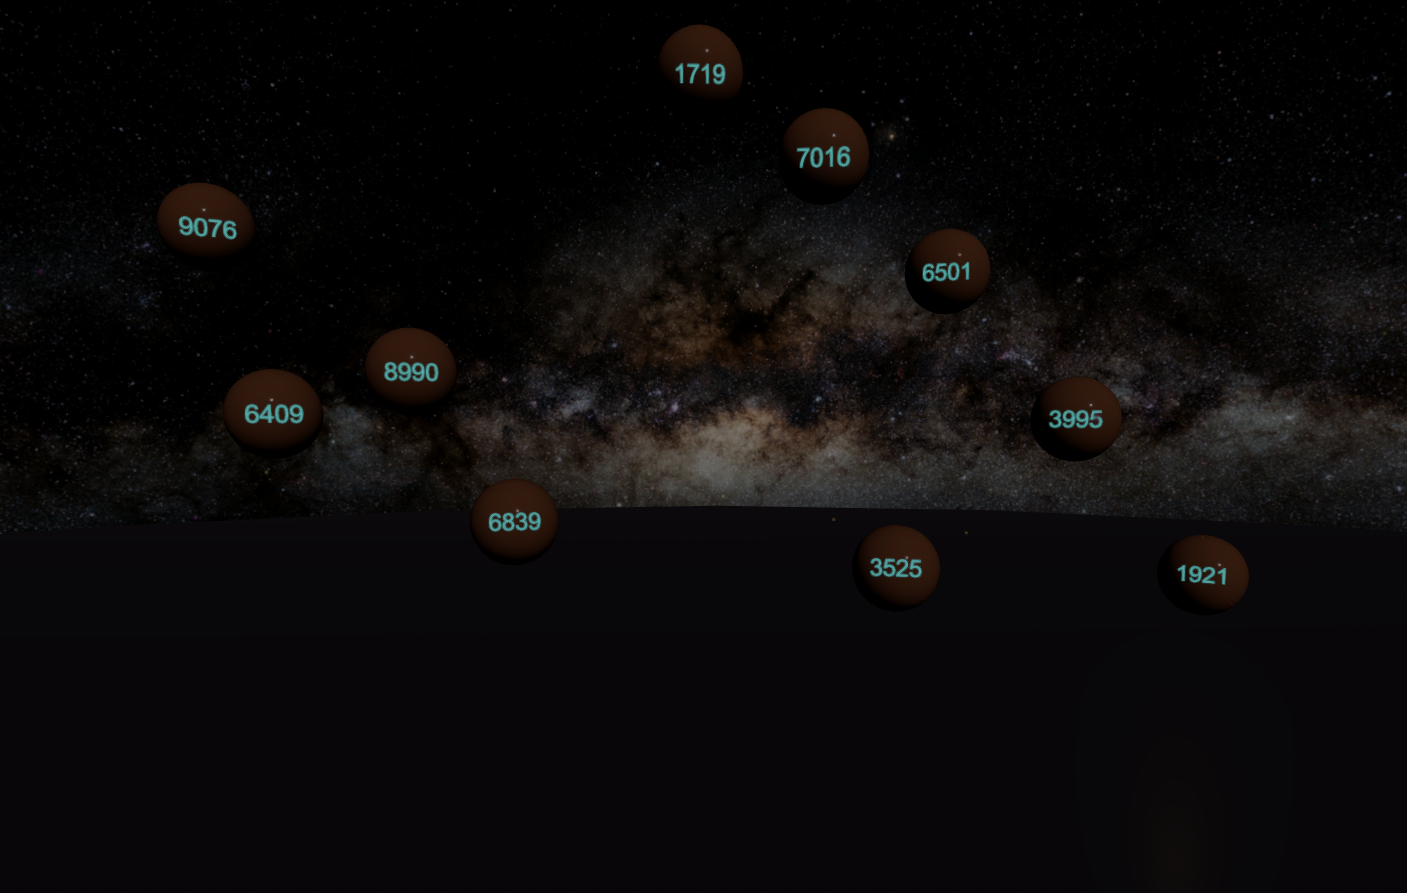
\includegraphics[width=0.8\textwidth]{./images/ordering.png}
	\caption{Erste Aufgabe der Studie. Der Text auf den Kugeln soll in aufsteigender Reihenfolge sortiert ausgewählt werden.}
	\label{fig:ordeing}
\end{figure}

\subsubsection{Stroop-Effekt} 
Im Mittelpunkt des Blickfeldes wird eine ausgeschriebene Farbe angezeigt. Die Textfarbe des Worts muss nicht zwangsläufig die der ausgeschriebenen Farbe sein. Der Proband soll als Eingabe die Textfarbe auswählen indem er mit dem Controller auf einem Interface die richtige Auswahl trifft. Beispiel kann in Figure~\ref{fig:stroop_test} gesehen werden. Diese Aufgabe dient dem Testen von ungewohnten Aufgaben, welche dem Anwender in der Regel nicht vertraut sind und auf welche sich der Proband in kürzester Zeit einstellen muss.

\begin{figure}
	\centering
	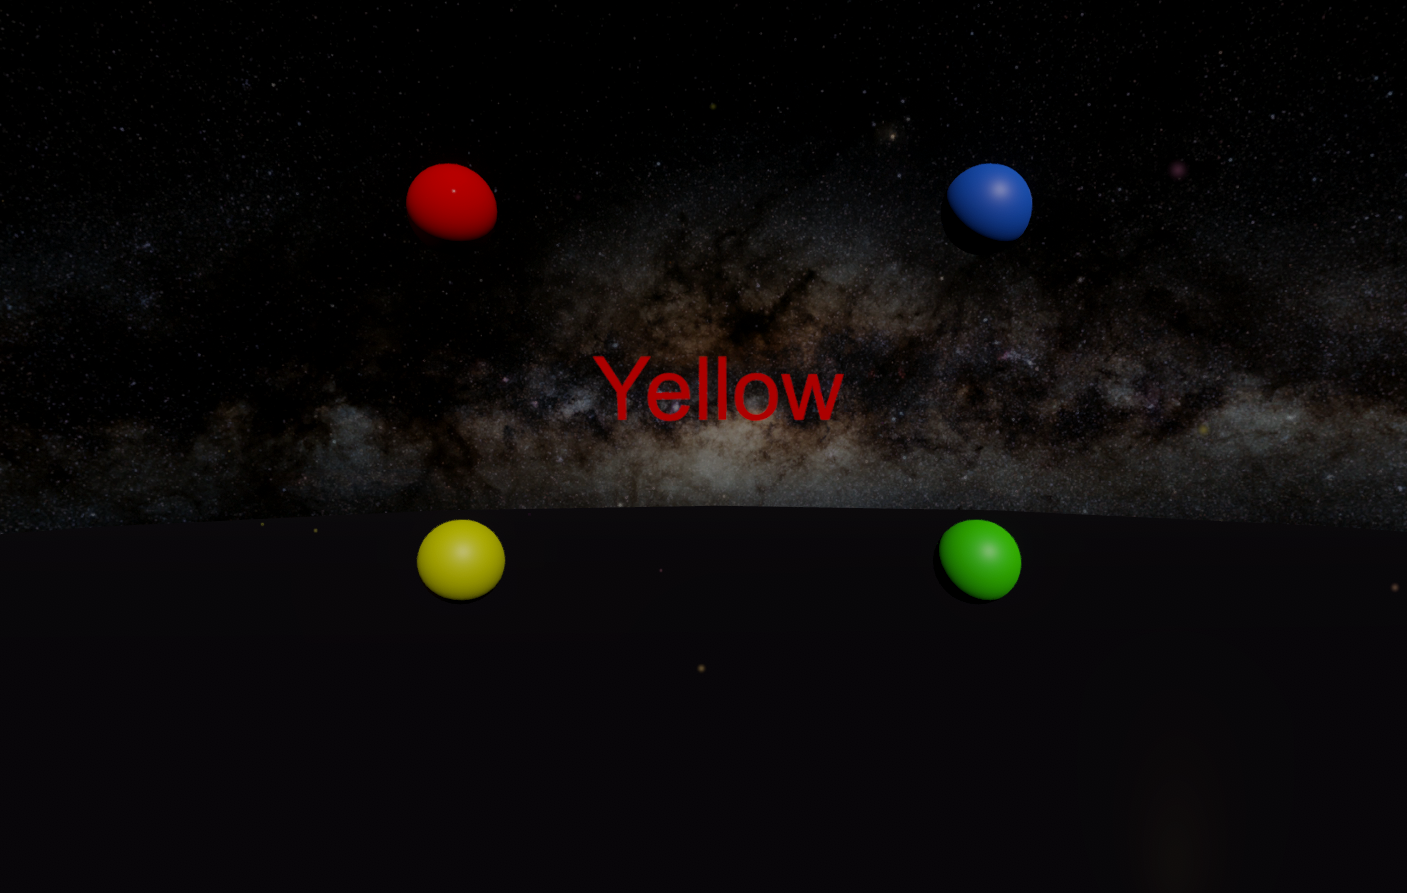
\includegraphics[width=0.8\textwidth]{./images/matching.png}
	\caption{Zweite Aufgabe. Teilnehmer der Studie sollen die Farbe, welche in Textform im Sichtbaren Bereich steht auswählen. Es soll nicht die gleiche Farbe ausgewählt werden.}
	\label{fig:matching}
\end{figure}

\subsubsection{Boxen zählen} 
In isometrischer Ansicht werden eine Vielzahl von Boxen innerhalb der virtuellen Umgebung angezeigt. Die Boxen stehen aufeinander und verdecken zum Teil den Blick auf andere Boxen. Es soll durch die Schlussfolgerung, dass diese, so wie in der realen Welt, nicht in der Luft schweben können, die Anzahl der Boxen gezählt und ausgewählt werden. Diese Aufgabe konzentriert sich auf das räumliche Wahrnehmen und Vorstellungsvermögen des Anwenders.

\begin{figure}
	\centering
	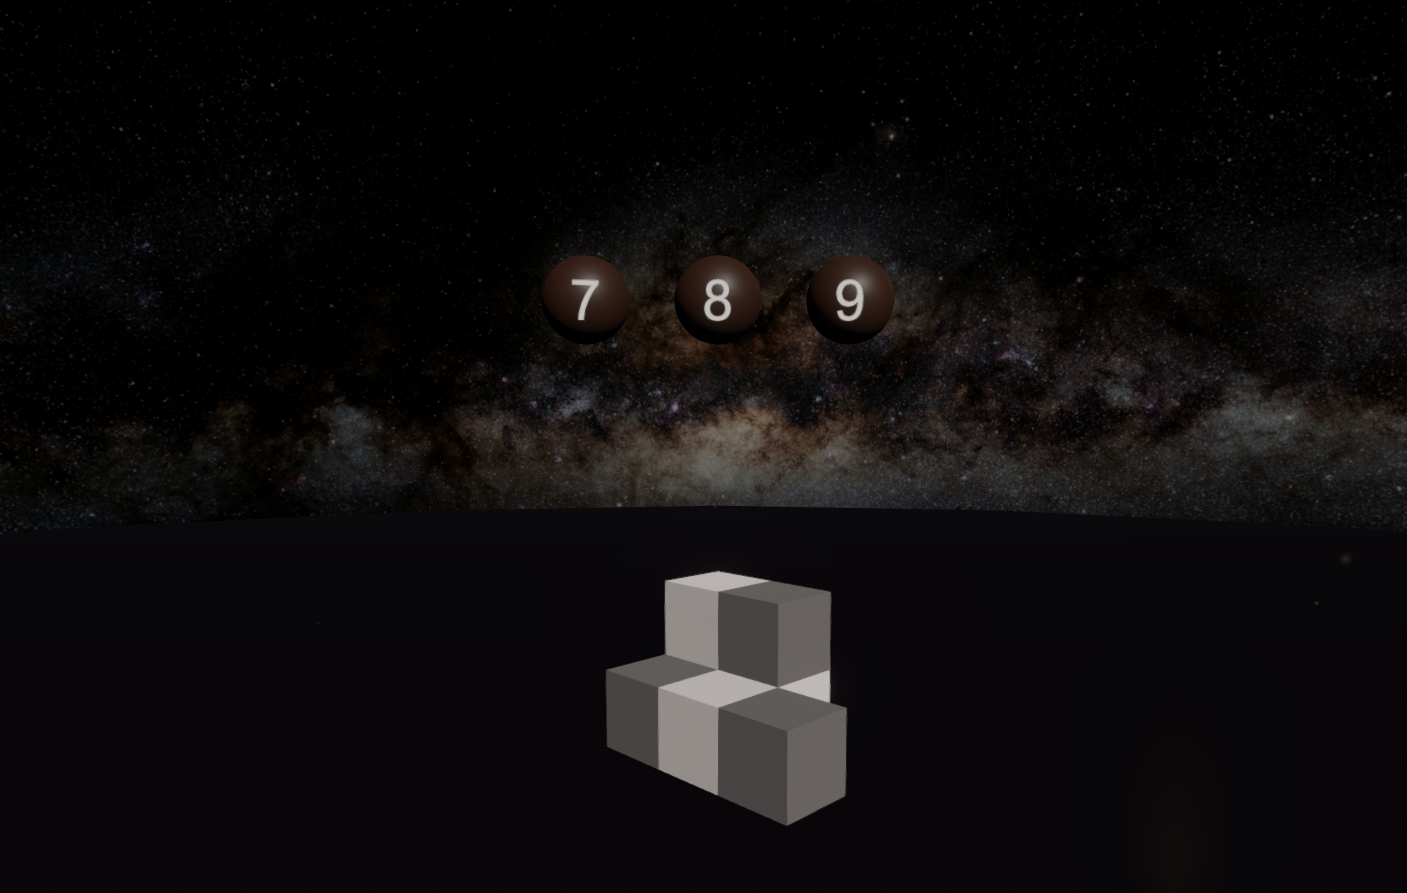
\includegraphics[width=0.8\textwidth]{./images/counting.png}
	\caption{Dritte Aufgabe in der virtuellen Umgebung. Die Teilnehmer sollen die Anzahl der Boxen zählen. Boxen verdecken die Sicht auf andere Boxen. Sie können nicht in der Luft schweben.}
	\label{fig:counting}
\end{figure}

\subsection{Studienumgebung}
\todoSab{Hier bitte die Räumlichkeiten kurz beschreiben, also Raum, Licht, Störfaktoren etc.}

%  ===== THIS IS INTENTIONALLY LEFT HERE AS REFERENCE FOR SUBFIGURES (copy&paste)
% \begin{figure}
% 	% \centering
% 	\begin{subfigure}{0.4\textwidth}
% 		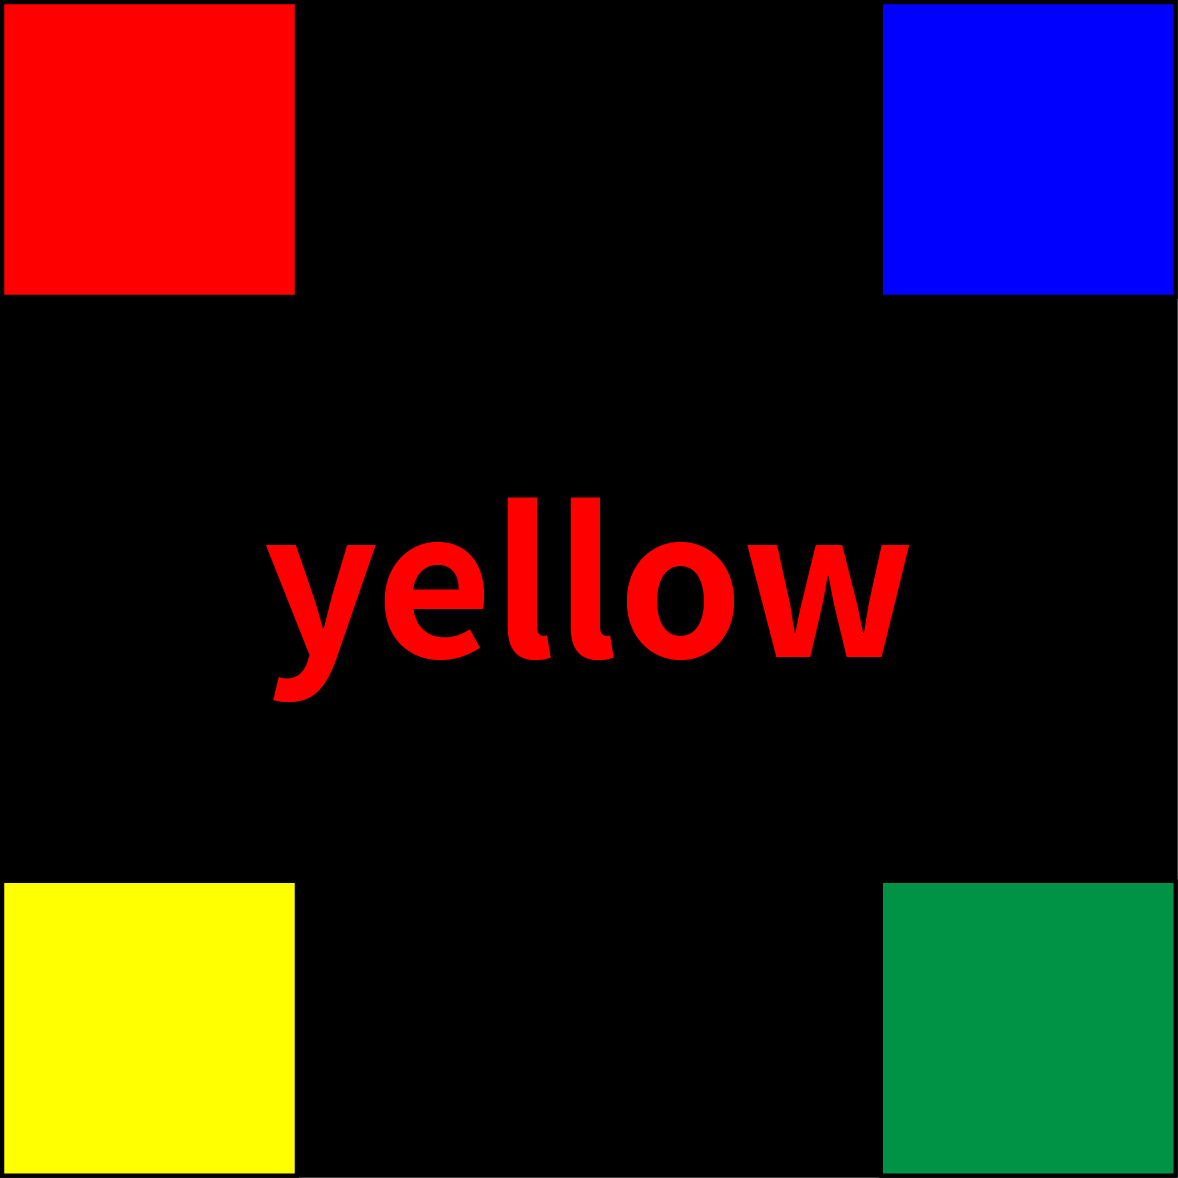
\includegraphics[width=\textwidth]{./images/Reversed_stroop_test.jpg}
% 		\caption{Stroop Test, ElvisLin CC BY-SA 4.0. \url{https://commons.wikimedia.org/wiki/File:Reversed_stroop_test.jpg}} % subcaption
% 		\label{fig:stroop_test}
% 	\end{subfigure}%
% 	\hfill
% 	\begin{subfigure}{0.5\textwidth}
% 		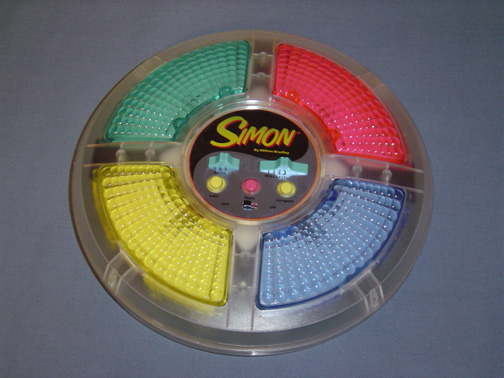
\includegraphics[width=\textwidth]{./images/Simon_game.jpg}
% 		\caption{Senso / Simon, Larry D. Moore CC BY-SA 3.0. \url{https://commons.wikimedia.org/wiki/File:Simon_game.jpg}} % subcaption
% 		\label{fig:simon}
% 	\end{subfigure}
% 	\caption{Beispiele für die Spiele mit denen die Teilnehmer konfrontiert werden.} % caption for whole figure
% \end{figure}


\chapter{Implementierung}
Auf Softwareseite soll eine digitale Umgebung mittels Unity 3D\footnote{~Unity3D~\url{https://unity3d.com}} erstellt werden. Das gewählte Interface zur Untersuchung der beschriebenen Problemstellung ist die HTC Vive\footnote{~HTC Vive~\url{https://www.vive.com}} mit den zugehörigen Controllern. Bewegung innerhalb der digitalen Umgebung ist, bis auf Kopfbewegungen, nicht vorgesehen, da die Probanden in einem sitzenden Zustand untersucht werden. Die Eingabemethoden zur Bewältigung der gestellten Aufgaben werden mit Zeigeoperationen innerhalb der virtuellen Umgebung realisiert. Eine Implementierung zum Nachverfolgen der Augenbewegung von Probanden (Eye-Tracking) wird nicht selbst durchgeführt, sondern auf bestehende Implementierungen zurückgegriffen. 

Fragebögen werden über das Limesurvey online Fragebogen Tool der Universität Ulm\footnote{~Limesurvey~\url{https://surveys.informatik.uni-ulm.de/limesurvey/
}} gestellt und beantwortet. 


\chapter{Durchführung der Studie}

\section{Zeitplan}
Die Daten beziehen sich auf den Zeitpunkt zu dem der jeweilige Schritt abgeschlossen sein sollte.
\begin{itemize}
    \item \textbf{Dezember 2018} Recherche bestehender Forschung
    \item \textbf{Dezember 2018} Digitale Umgebung in Unity3D erstellen und mit erster Testphase validieren
    \item \textbf{Januar 2018} Erste Studie durchführen
    \item \textbf{Februar 2019} Auswertung der durchgeführten Studie.
    \item \textbf{März 2019} Entwurf der zweiten Studie
    \item \textbf{April 2019} Erweiterte Umgebung in Unity3D erstellen und für den zweiten Studiendurchlauf vorbereiten
    \item \textbf{Mai 2019} Durchführung der zweiten Studie für erweiterte Ergebnisse
    \item \textbf{Juni 2019} Auswertung der Ergebnisse von zweiter Studie
    \item \textbf{September 2019} Dokumentation der Ergebnisse und des Vorgehens
\end{itemize}

\section{Studiendesign}

\todoTob{das hier raus weil bei Lösungsansatz schon die Umgebung etc alles beschrieben wurde und das ja eher zu Vorarbeit zählt? Oder das aus Lösungsansatz hier rein?}

\section{Studiendurchführung}

Der Proband setzt sich in einen bequemen Stuhl, welcher von ihm nach Belieben verstellt werden kann. Nach kurzen Instruktionen zum Ablauf und zur Bedienung des VR-Controllers, wird dem Proband die VR-Brille aufgesetzt, woraufhin er als erstes in der virtuellen Umgebung einen SAM-Fragebogen ausfüllen muss. %sagt man dazu SAM-Fragebogen?
Bevor die eigentliche Studie beginnt, hat der Proband die Möglichkeit, sich ein wenig mit der Steuerung vertraut zu machen, indem er in der Umgebung den Controller verwendet, um schwebende Blasen platzen zu lassen, eine Mechanik die in allen drei späteren Aufgaben von elementarer Bedeutung sein wird. Sobald die Testperson durch das klicken auf einen Button angibt, bereit zu sein, beginnt die Schlafphase. Diese beträgt bei jedem einzelnen Probanden exakt 15 Minuten, jedoch wurde ihnen vor der Studie mitgeteilt, dass die Dauer zwischen 15 und 25 Minuten variiere. %Zeit nochmal checken
Bei unseren ersten 30 Teilnehmern wurde ein heller Lichtreiz verwendet um die Probanden aus dem Schlaf beziehungsweise aus ihrer Entspannung zu reißen. Bei 15 von ihnen dauerte es 20 Sekunden bis der Lichtreiz seine volle Helligkeit erreichte, wohingegen bei der anderen Hälfte der Lichtreiz fünf Sekunden benötigte um sich vollkommen zu entfalten.  Die restlichen 15 Probanden wurden nicht visuell, sondern durch das Geräusch einer Autoalarmanlage geweckt. %Zeiten checken!
Jeder Proband wurde innerhalb dieser Phase beobachtet, damit neben Informationen zum Stuhl (Winkel der Lehne) auch festgehalten werden konnte, wie unruhig beziehungsweise entspannt jeder einzelne von ihnen war. Ferner wurde jeder nach zehn Minuten nochmal genauer inspiziert, hierbei wurde die Atmung des Versuchsteilnehmers analysiert.
Bei allen 45 Testpersonen folgte nach dem Wecken die exakt identische Prozedur. Zunächst mussten sie auf einen Startbutton drücken um mit den Aufgaben zu beginnen. Die im Abschnitt 'Aufgaben' geschilderten Tasks wurden stets in derselben Reihenfolge von den Probanden abverlangt. Zuerst das Zahlen sortieren, gefolgt vom Farbspiel und zuletzt das zählen der Blöcke. %Noch überlegen, wie wir diese Spiele wirklich nennen wollen.
Sobald der Proband alle drei Aufgaben absolviert hat, muss er abermals den gleichen SAM-Fragebogen wie zuvor ausfüllen und darüber hinaus noch zusätzlich auf die Frage antworten, als wie anspruchsvoll er die gestellten Aufgaben erachtete.
Schlussendlich darf die VR-Brille abgesetzt werden, woraufhin der Proband als letztes noch an einer demographischen Umfrage, welche diesmal nicht in VR stattfindet, sondern an einem Computer im selben Raum, teilnimmt. Der Proband hat nun die gesamte Studie komplettiert.

\begin{figure}
	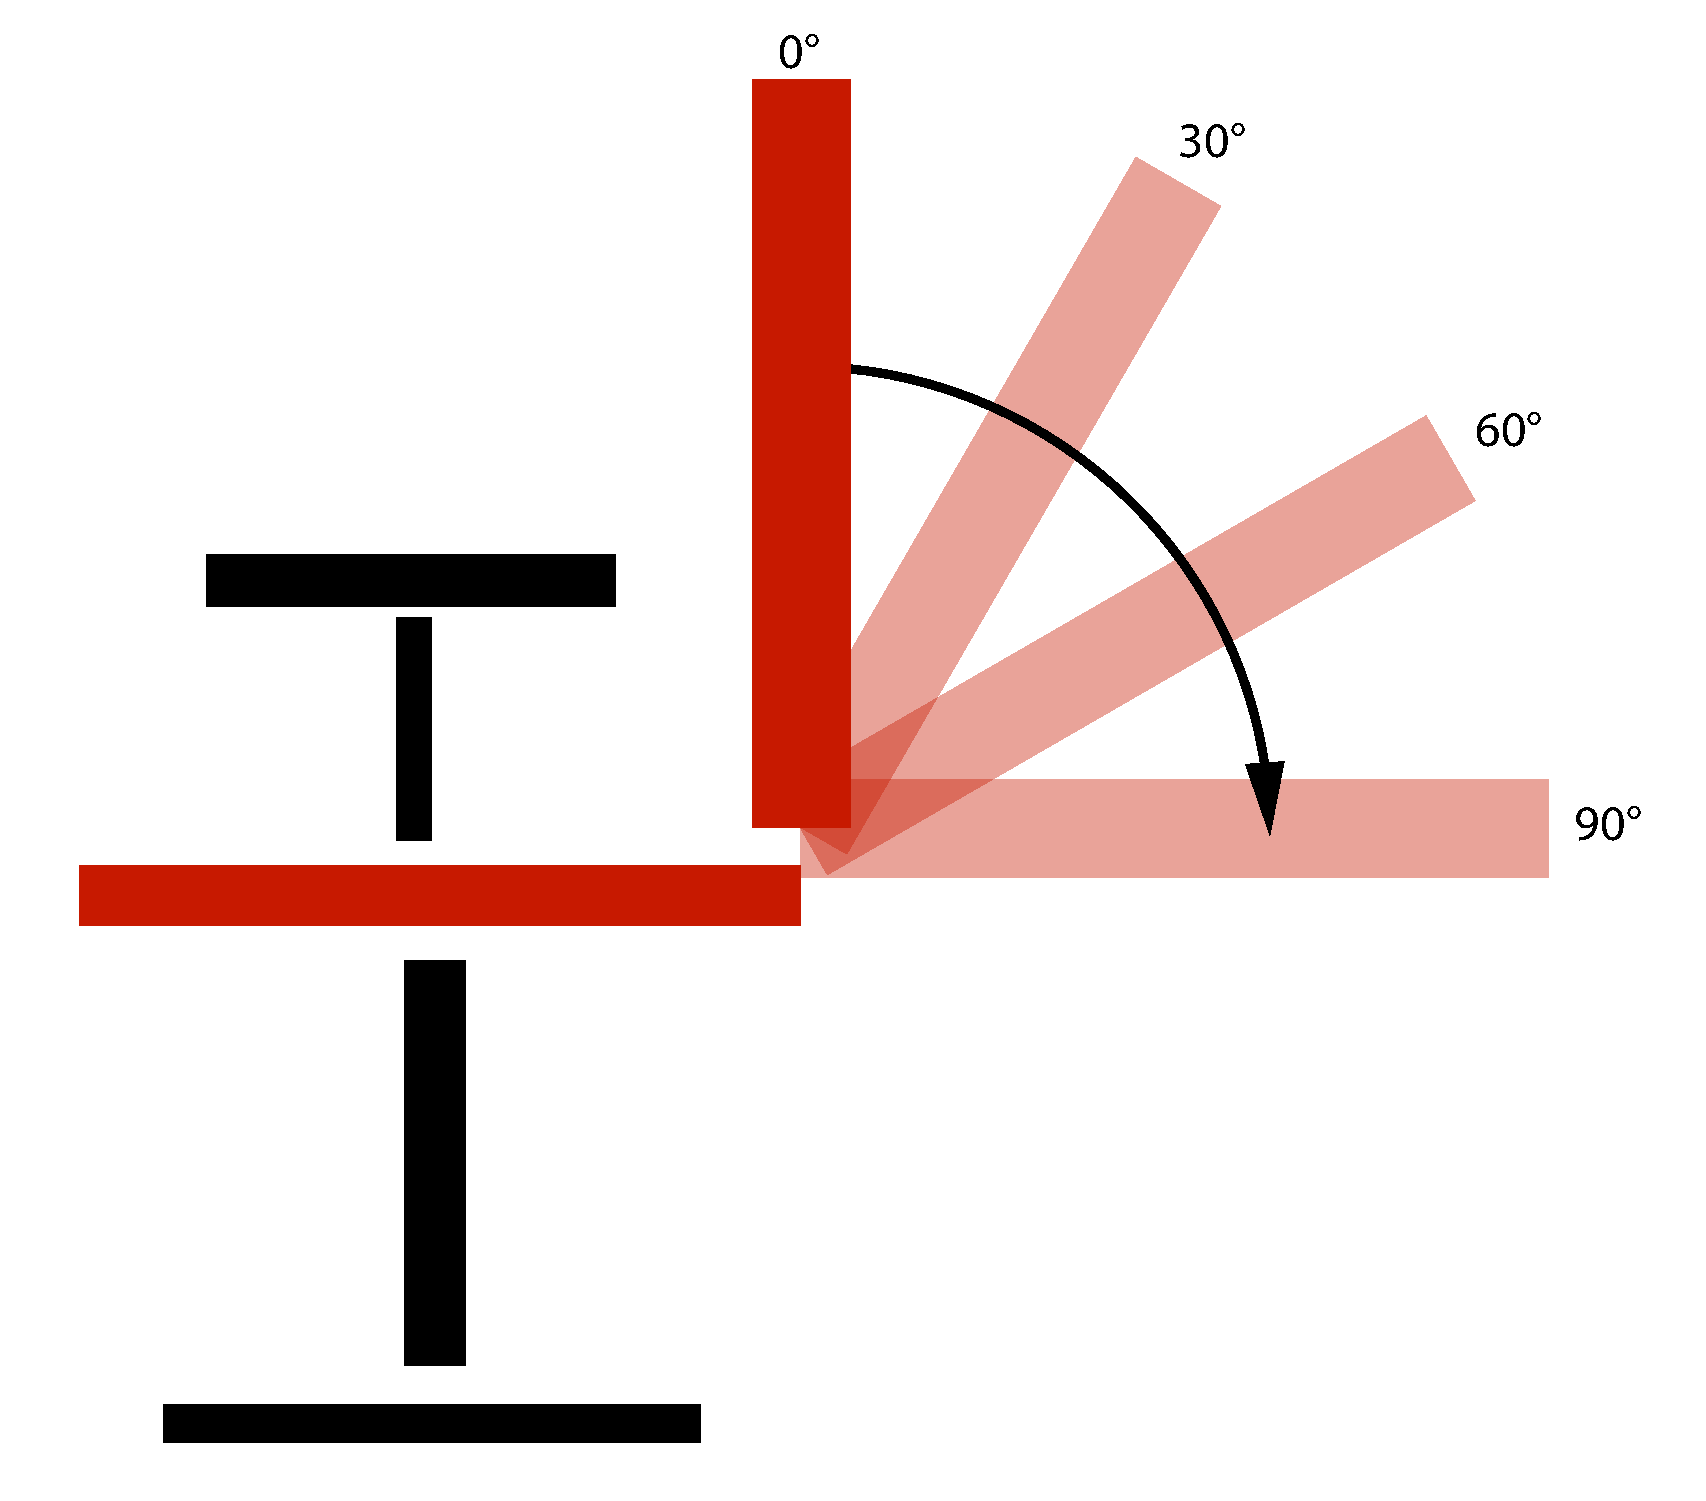
\includegraphics[width=0.8\textwidth]{./images/chair}
	\caption{Winkeleinstellungen vom verwendeten Stuhl in der Studie}
	\label{fig:counting}
\end{figure}

\todoSab{Könnt ihr hier eine Tabelle erstellen für das, wie Oft eine jeweilige einstellung vom Stuhl vorgekommen ist?? Dann kann man das visualisieren.}
\todoLuc{Könnt ihr hier eine Tabelle erstellen für das, wie Oft eine jeweilige einstellung vom Stuhl vorgekommen ist?? Dann kann man das visualisieren.}

\section{Ergebnisse}

Unsere Studie wurde vom 04. Juni bis zum 18. August 2019 durchgeführt. Es nahmen insgesamt 45 Teilnehmer in zwei Durchläufen teil. Der erste Durchlauf erfasste zwei Gruppen, dessen geänderter Parameter die Zeit war, in der ein Licht innerhalb der virtuellen Umgebung die Probanden 'geweckt' hat. Im zweiten Durchlauf wurde dieser Parameter geändert und die Teilnehmer wurden mit einem Ton geweckt, wie man ihn als Hinweiston in modernen Autos wiederfindet. Hierbei wurde die Zeit, in der die Studienteilnehmer den Ton selbständig abgeschaltet haben gemessen. Zusätzlich zur Interaktionen zwischen Proband und VR System wurden noch einige demografische und personenbezogene Fragen außerhalb der VR Umgebung gestellt, welche zusätzlich aufgelistet werden.

\subsection{Demografische Ergebnisse}

Es waren von den 45 Teilnehmern nach eigenen Angaben 12 weiblich, 33 männlich und 0 Divers. Eine grafische Repräsentation kann in Abbildung~\ref{fig:gender} und die zugehörigen Zahlenwerte in Tabelle~\ref{tab:sc_results_gender} eingesehen werden. Die Teilnehmer haben eine große Bandbreite an Studiengängen abgedeckt, welche neben diversen Naturwissenschaften auch beispielsweise Informatik, Wirtschaftsmathematik und Psychologie beinhalteten. Diese können in Tabelle~\ref{tab:sc_results_study} entnommen werden können.

\begin{figure}[H]
	\centering
	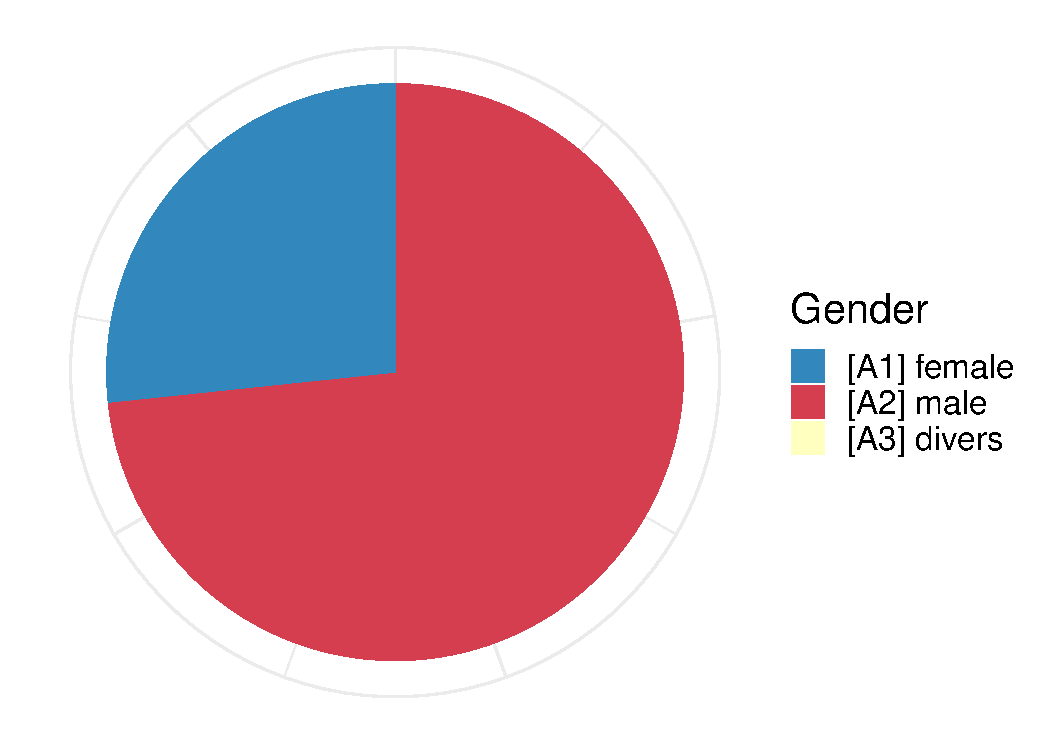
\includegraphics[width=0.75\textwidth]{./_StudyResults/gender}
	\caption{Geschlechterverteilung der Studienteilnehmer}
	\label{fig:gender}
\end{figure}

Das Alter der Teilnehmer reichte von 19 bis 30 Jahren, wobei der Median bei 23 und der Mittelwert bei 23,04 Jahren mit einer Standardabweichung von 2.53 lag. Eine grafische Darstellung kann in Abbildung~\ref{fig:age} und die zugehörigen Zahlenwerte in Tabelle~\ref{tab:sc_results_age} gesehen werden.

\begin{figure}[H]
	\centering
	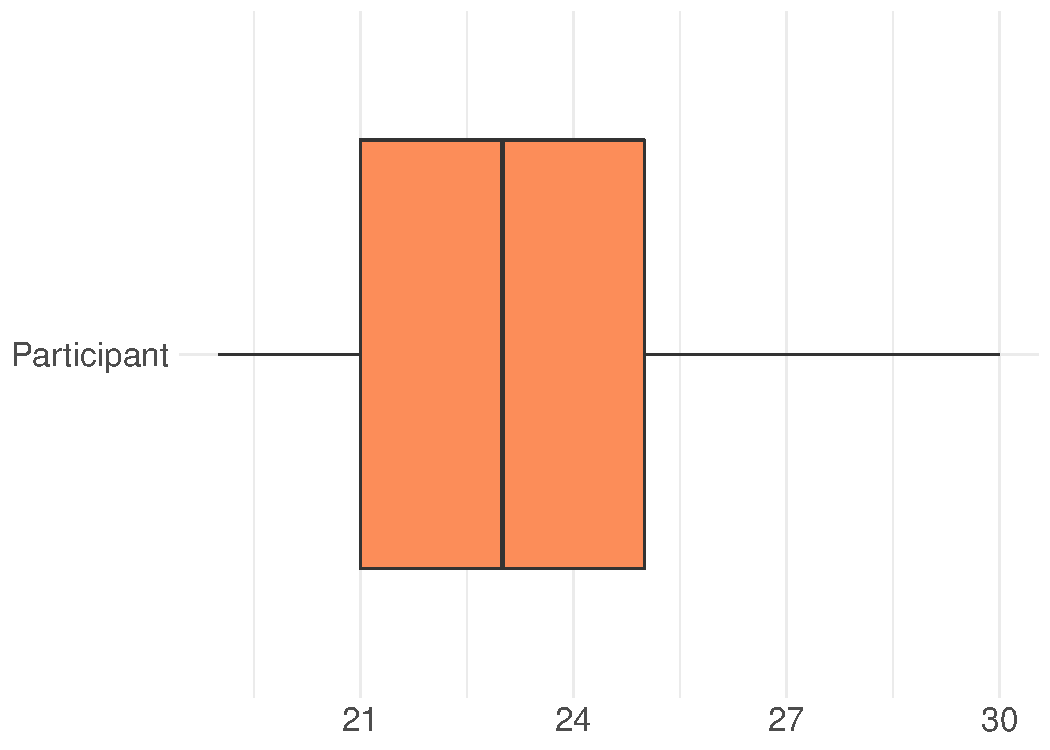
\includegraphics[width=0.75\textwidth]{./_StudyResults/age}
	\caption{Boxplot des Alters der Studienteilnehmer}
	\label{fig:age}
\end{figure}

Die Teilnehmer gaben an, dass sie unterdurchschnittlich wenig Erfahrung mit virtueller Realität haben. Hierbei lag der Mittelwert bei 2,93 von 7 möglichen Punkten. Die Standardabweichung beträgt 1,78. Die Ergebnisse können auch in Tabelle~\ref{tab:sc_results_expVR} und Tabelle~\ref{tab:sc_numbers_expVR} angesehen werden. Bei augmentierter Realität sehen wir ein ähnliches Abbildung. Hier gaben die Teilnehmer an einen durchschnittlichen Erfahrungswert von 2.36 von 7 zu haben. Die Standardabweichung in diesem Fall beträgt 1,38. Außerdem ist noch hervorzuheben, dass keiner der Befragten einen Wert von 7 ausgewählt hat. Die Ergebnisse hierzu können in Tabelle~\ref{tab:sc_results_expAR} und Tabelle~\ref{tab:sc_numbers_expAR} eingesehen werden, zusätzlich existiert eine grafische Repräsentation in den Abbildungen~\ref{fig:expVr} und~\ref{fig:expAr}.

\begin{figure}[H]
	\centering
	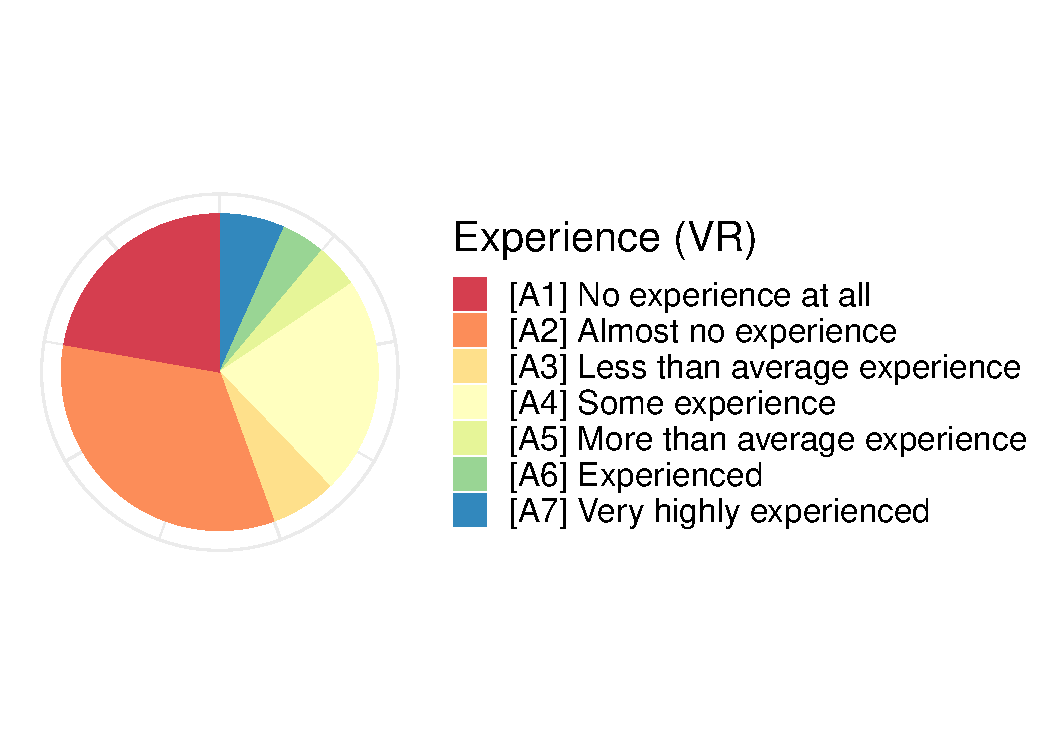
\includegraphics[width=0.75\textwidth]{./_StudyResults/expVr}
	\caption{Grafische Repräsentation der Antworten zur Frage "`How much experience do you have with VR?"'.}
	\label{fig:expVr}
\end{figure}%
\begin{figure}[H]
	\centering
	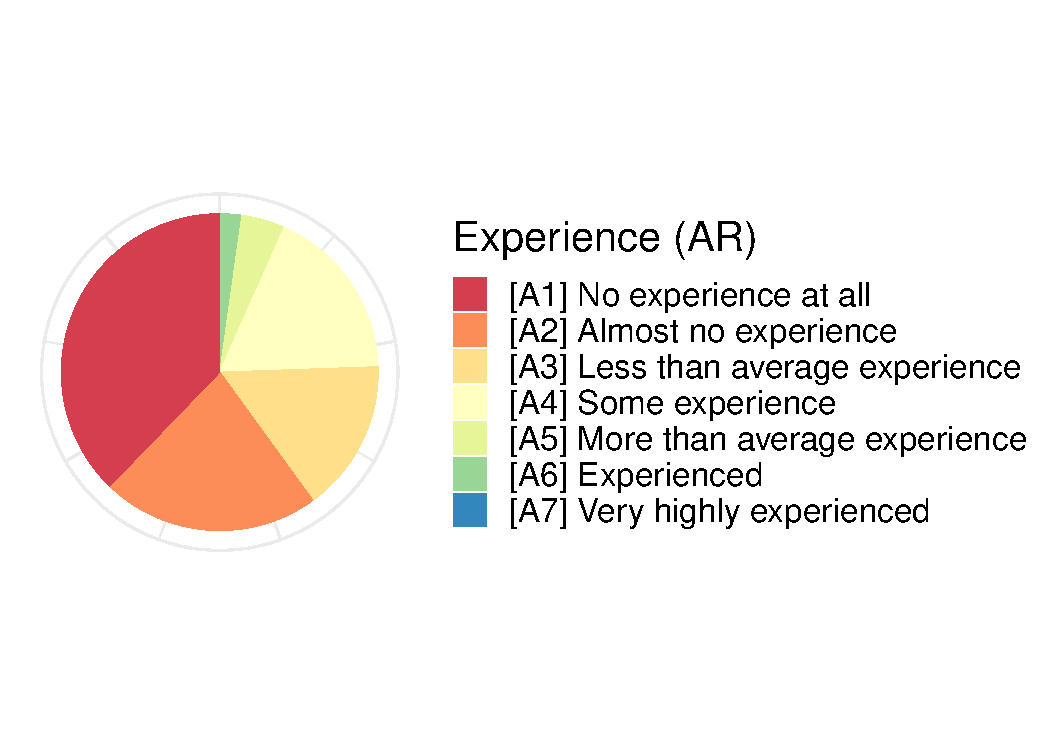
\includegraphics[width=0.75\textwidth]{./_StudyResults/expAr}
	\caption{Grafische Repräsentation der Antworten zur Frage "`How much experience do you have with AR?"'.}
	\label{fig:expAr}
\end{figure}

\subsection{Umgebungsvariablen}
\subsubsection{Stuhleinstellungen}

Die Umgebung der Studie wurde so abgeschottet gewählt, dass wenig äußere Einflüsse störend auf den Studienablauf wirken konnten. Trotz dieser Platzwahl bekamen wir Rückmeldung durch die Probanden, dass sie die Umgebung nicht perfekt zum Einschlafen gewählt wurde. Weitere Kommentare der Nutzer zur Bequemlichkeit der VR Brille, als auch zum Stuhl, sowie allen weiteren Umgebungsvariablen können im Anhang gefunden werden.

Die durchschnittliche Neigung der Stuhllehne lag über alle Durchläufe bei 38,6$^\circ$. Eine genaue Auflistung der Einstellungen kann in Tabelle~\ref{tab:sc_results_chair} eingesehen werden. Hierbei ist zu beachten, dass die Werte vom Studienbetreuer zur Zeit der Ruhephase subjektiv notiert wurden. Außerdem ist zu beachten, dass die Winkeleinstellung mit einer Abweichung notiert worden sein kann. Hierdurch ergeben sich die hier aufgeführten Ergebnisse. Die möglichen Einstellung des verwendeten Stuhls können in Abbildung~\ref{fig:chair_backrest} gefunden werden.

\begin{figure}[H]
	\centering
	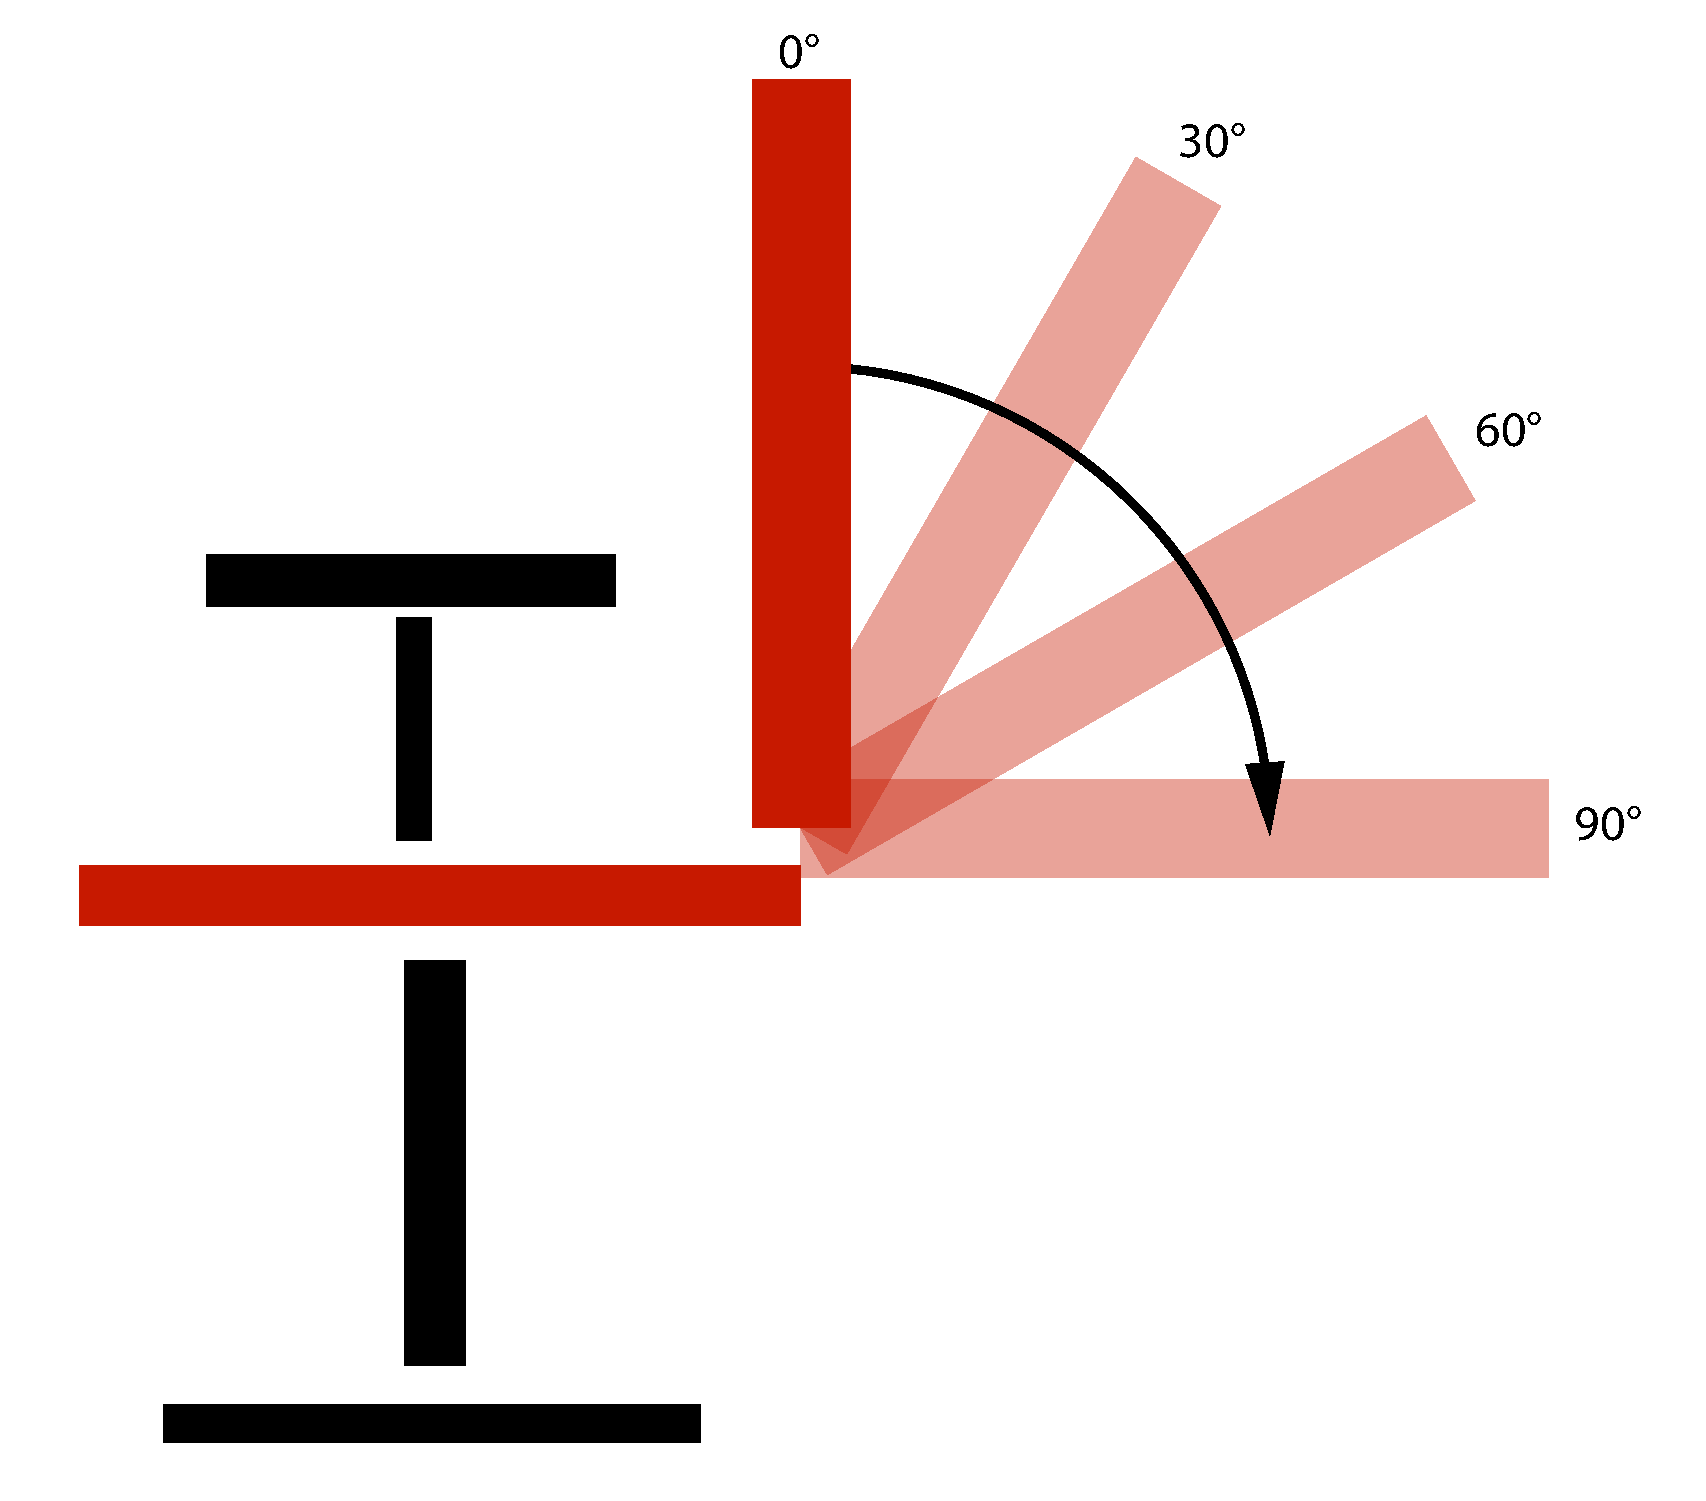
\includegraphics[width=0.75\textwidth]{./images/chair}
	\caption{Winkeleinstellungen vom verwendeten Stuhl in der Studie}
	\label{fig:chair_backrest}
\end{figure}


\subsubsection{Dauer des Wecker-Tons}

Die Probanden die mit Ton geweckt wurden, hatten einen Button der den Aufwachteil der Zeitmessung beendet hat. Diese Zeiten reichten von 3.91 bis 10.84 Sekunden. Der Median des Ton-Abstellens beträgt 5.87 Sekunden, also betätigten die meisten Teilnehmer ca. nach 6 Sekunden den Button der sie zur ersten Aufgaben weitergeleitet hat. 

\begin{figure}[H]
	\centering
	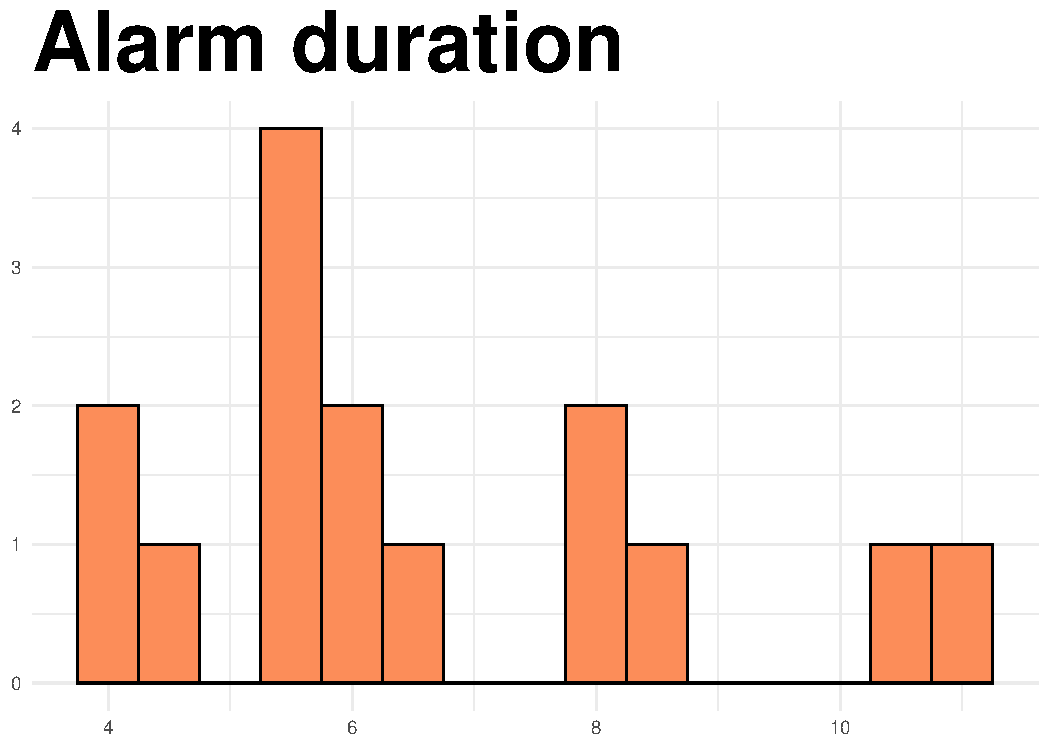
\includegraphics[width=0.75\textwidth]{./_StudyResults/alarmDurationHist}
	\caption{Histogramm der Zeit (s), wie lange die Teilnehmer der Studie den Wecker-Ton laufen ließen. Genauigkeit: 500ms}
	\label{fig:alarmDurationHist}
\end{figure}

\subsection{Aufgabenergebnisse} 

Ein Hauptaspekt der Studie liegt auf der Aufgabenbewältigung und vor allem darauf, wie gut diese gelöst werden können unter den uns bekannten Einflüssen. 

\subsubsection{Fehlerraten}

Die Unterteilung in unsere 3 Gruppen, die wir untersucht haben, lässt sich im Folgenden so verstehen, dass die Gruppe \textit{Fade 5}, die Gruppe mit 5 FadeSeconds beim Aufwachen ist und die zweite Gruppe \textit{Fade 20} die mit 20 Sekunden FadeSeconds ist. Als dritte Studiengruppe haben wir die Gruppe \textit{Alarm}, bei welcher die Probanden durch den Weckton geweckt wurde.

Für die erste Aufgabe gilt, dass ein Fehler dann als Fehler gewertet wird, wenn danach eine kleinere Zahl vorkommt. Eine ausgewählte Reihenfolge $3, 2, 1$ zählt also als 3 Fehler insgesamt, da $3 > 2 > 1$ (2 Fehler) sowie $2 > 1$ (1 Fehler). Auf diese Weise kommen auch 45 Fehler zustande; und zwar dann, wenn alle Zahlen falsch herum ausgewählt wurden. Dies entspricht der Summe von 1 bis 9.
Wie in Tabelle~\ref{fig:orderingMistakeHistogram} abzulesen, haben nur knapp 58\% der Studienteilnehmer überhaupt keine Fehler begangen. Häufig wurden vereinzelte Fehler gemacht, welche die Teilnehmer direkt beim Ausführen der Aufgabe bemerkten, was meist durch verbale oder physische Reaktionen deutlich wurde. 
Eine Fehlerzahl von 44 oder 45 wurde dann erreicht, wenn die Probanden gedacht haben, sie sollen die Zahlen genau andersherum sortieren, wie uns im Nachhinein mehrere Nutzer mitgeteilt haben.
Aus der Gruppe Fade 5 haben am Meisten mit 0 Fehlern abgeschnitten. Die schlechtesten Ergebnisse stammen aus der Alarm Gruppe, wie in Abbildung~\ref{fig:orderingMistakeHistogram} erkennbar ist. \todoAll{mehr Fehler Aufg 1 beschreiben?}

\begin{figure}[H]
	\centering
	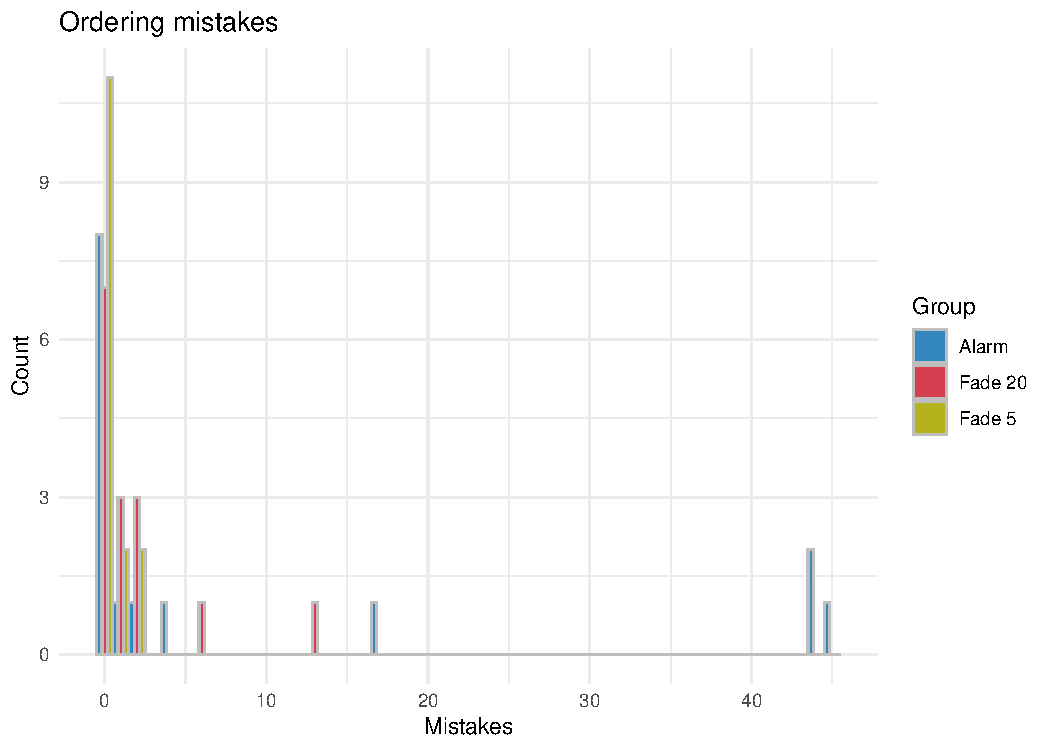
\includegraphics[width=0.75\textwidth]{./_StudyResults/orderingMisHist}
	\caption{Häufigkeit der Fehler unterteilt in Gruppen in Aufgabe 1: Zahlenfolge. Darstellungsgenauigkeit: 1}
	\label{fig:orderingMistakeHistogram}
\end{figure}

\begin{table*}
	\caption{Vorkommnisse der Fehler unterteilt in Gruppen in Aufgabe 1: Zahlenfolge.}~\label{tab:orderingMistakeNumbers}
	
	\setlength\tabcolsep{3pt}
	\renewcommand{\arraystretch}{1.4}% for the vertical padding
	\begin{tabularx}{\textwidth}{ | l | x | x | x | x | x | x | x | x | x | }
		\hline
		Anzahl Fehler & 0   & 1  & 2  & 4  & 6  & 13 & 17 & 44  & 45 \\ \hline\hline
		Alarm 	  & 8  & 1  & 1  & 1  & 0  & 0  & 1  &  2  & 1  \\ \hline
		Fade 20	  & 7  & 3  & 3  & 0  & 1  & 1  & 0  &  0  & 0  \\ \hline
		Fade 5	  & 11  & 2  & 2  & 0  & 0  & 0  & 0  &  0  & 0  \\ \hline
	\end{tabularx}
\end{table*}

In Aufgabe 2 ist ein Fehler dann gegeben, wenn das ausgewählte Feld nicht dem gefordertem Feld entspricht, also ist das Maximum 10.
Von ca 73\% wurde diese Aufgabe komplett fehlerfrei gelöst.
Auch hier wurden Fehlerzahlen die 8 oder höher waren dann erzielt, wenn die Aufgabe so verstanden wurde, dass die Farbe in der das Wort geschrieben stand gewählt wurde.
Aus Abbildung~\ref{fig:matchingMistakeHistogram} ist deutlich ablesbar, dass aus den Gruppen Alarm und Fade 5 gleich viele Fehler gemacht haben. Bis auf ein paar Probanden die die Aufgabe nicht komplett richtig bearbeitet haben weißt die dritte Gruppe Fade 20 keine Unterschiede auf.

\todoTob{nicht gut ablesbar, wo die Blaken dazugehören, also bspw zweiter roter von links hat der mit dem blauen daneben zu tun oder nicht? vielleicht so kleine schwarze striche an der x achse die zeigen hier ist ein schritt? Und bei mistakes steht bei der x achse 2.5 das ist glaub verwirrend weil gibt ja keine halben fehler}

\begin{figure}[H]
	\centering
	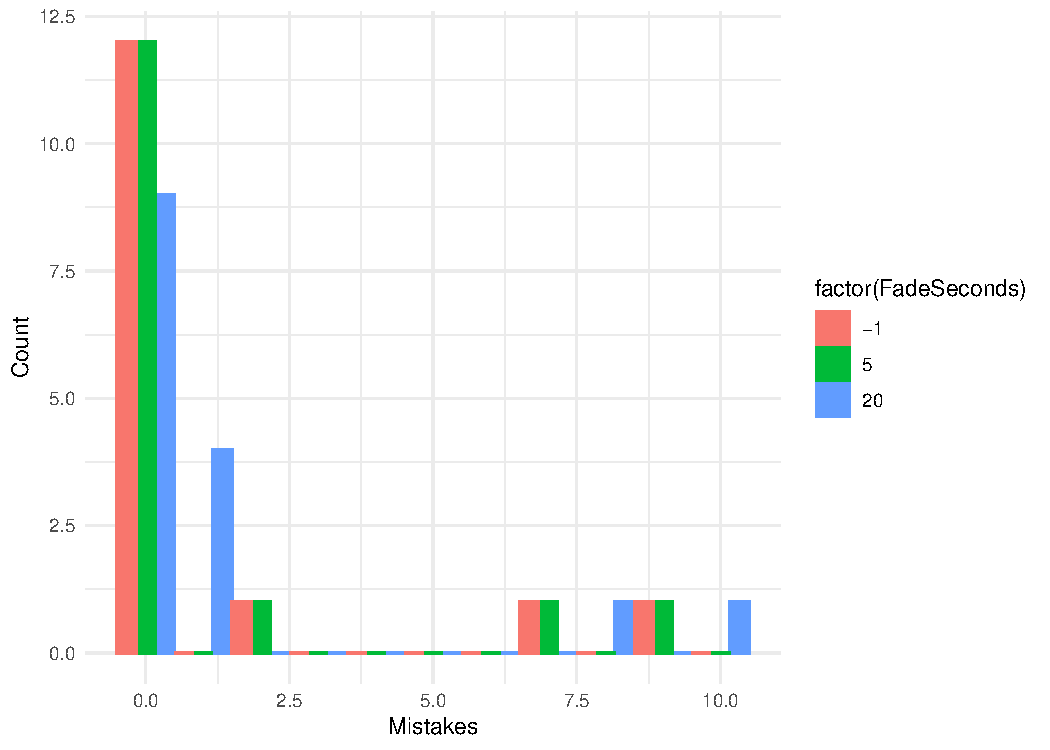
\includegraphics[width=0.75\textwidth]{./_StudyResults/matchingMisHist}
	\caption{Häufigkeit der Fehler unterteilt in Gruppen in Aufgabe 2: Stroop-Effekt. Darstellungsgenauigkeit: 1}
	\label{fig:matchingMistakeHistogram}
\end{figure}

\begin{table*}
	\caption{Vorkommnisse der Fehler unterteilt in Gruppen in Aufgabe 2: Stroop-Effekt.}~\label{tab:matchingMistakeNumbers}
	
	\setlength\tabcolsep{3pt}
	\renewcommand{\arraystretch}{1.4}% for the vertical padding
	\begin{tabularx}{\textwidth}{ | l | x | x | x | x | x | x | x | }
		\hline
		Anzahl Fehler & 0   & 1  & 2  & 7  & 8  & 9 & 10 \\ \hline\hline
		Alarm 	  & 12  & 0  & 1  & 1  & 0  & 1 & 0  \\ \hline
		Fade 20   & 9  & 4  & 0  & 0  & 1  & 0 & 1  \\ \hline
		Fade 5 	  & 12  & 0  & 1  & 1  & 0  & 1 & 0  \\ \hline
	\end{tabularx}
\end{table*}

In Aufgabe 3 zählt ein Fehler dann, wenn nicht die richtige Anzahl von den gegebenen Auswahlmöglichkeiten gewählt wurde. Die maximale Anzahl an Fehlern ist bei 3 Durchläufen also drei.
Von knapp 75\% wurde diese Aufgabe fehlerfrei gemeistert und kein Proband hat alle 3 Boxenzahlen falsch bestimmt. Die durchschnittliche Fehleranzahl beträgt 0.31, was unter Anderem im Anhang in Tabelle~\ref{tab:sc_results_counting} nachzulesen ist.
Aus Abbildung~\ref{fig:countingMistakeHistogram} ist gut erkennbar, dass die Alarm Gruppe höchstens einen Fehler gemacht hat, wohingegen die Licht Gruppen jeweils auch Probanden haben, die zwei Fehler gemacht haben. Zudem haben die Licht Gruppen beide die höchste Anzahl an Probanden, die die Aufgabe fehlerlos gelöst haben.

\begin{figure}[H]
	\centering
	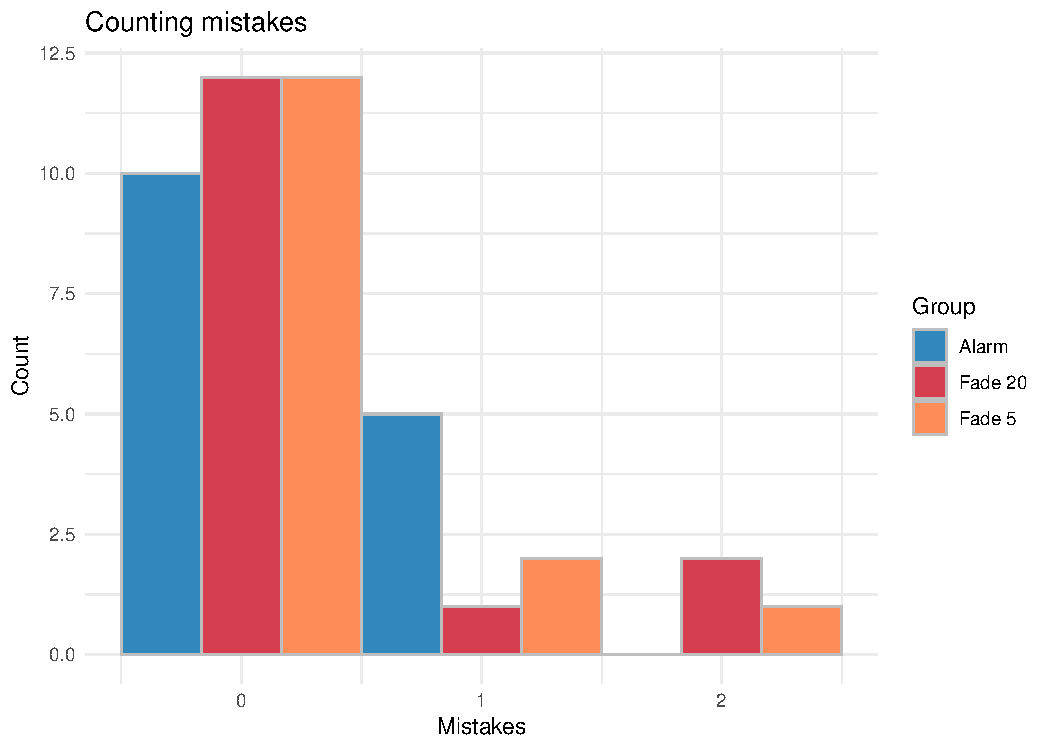
\includegraphics[width=0.75\textwidth]{./_StudyResults/countingMisHist}
	\caption{Häufigkeit der Fehler unterteilt in Gruppen in Aufgabe 3: Boxen zählen. Darstellungsgenauigkeit: 1}
	\label{fig:countingMistakeHistogram}
\end{figure}

\begin{table*}
	\caption{Vorkommnisse der Fehler in Aufgabe 3: Boxen zählen.}~\label{tab:countingMistakeNumbers}
	
	\setlength\tabcolsep{3pt}
	\renewcommand{\arraystretch}{1.4}% for the vertical padding
	\begin{tabularx}{\textwidth}{ | l | x | x | x | }
		\hline
		Anzahl Fehler & 0   & 1  & 2 \\ \hline\hline
		Alarm 	  & 10  & 5  & 0 \\ \hline
		Fade 20   & 12  & 1  & 2 \\ \hline
		Fade 5 	  & 12  & 2  & 1 \\ \hline
	\end{tabularx}
\end{table*}

\subsubsection{Benötigte Zeit für die Aufgabenerledigung}

Die jeweils gemessene Zeit erstreckt sich über den Start, der mit der Erklärung der Aufgabe gekennzeichnet wird, bis hin zum Ende der Zeitmessung, was den Abschluss der Aufgabe bedeutet.

Die Zeit, die für das Erledigen von Aufgabe 1 benötigt wurde, hat ihr Minimum bei 16.59 Sekunden. Die Anzahl der Teilnehmern die in einem Bereich von 2-Sekundenschritten, angefangen bei 15-17 Sekunden fertig geworden sind können in Abbildung~\ref{fig:orderingTimeHistogram} abgelesen werden. Die meistbenötigte Zeit 42.49 Sekunden, sowie ein Durchschnitt von 26.80 Sekunden können aus Tabelle~\ref{tab:times_results_ordering} entnommen werden.
In der Fade 5 Gruppe gibt es breit verteilte Erledigungszeiten zwischen 16 und 43 Sekunden, wohingegen sich die anderen beiden Gruppen im 20 bis 40 Sekunden Bereich aufhalten. Wie in Abbildung~\ref{fig:orderingTimeHistogram} zu erkennen ist, gibt es in der Alarm Gruppe einen Häufungspunkt bei der benötigten Zeit um die 20 Sekunden Grenze herum.

\begin{figure}[H]
	\centering
	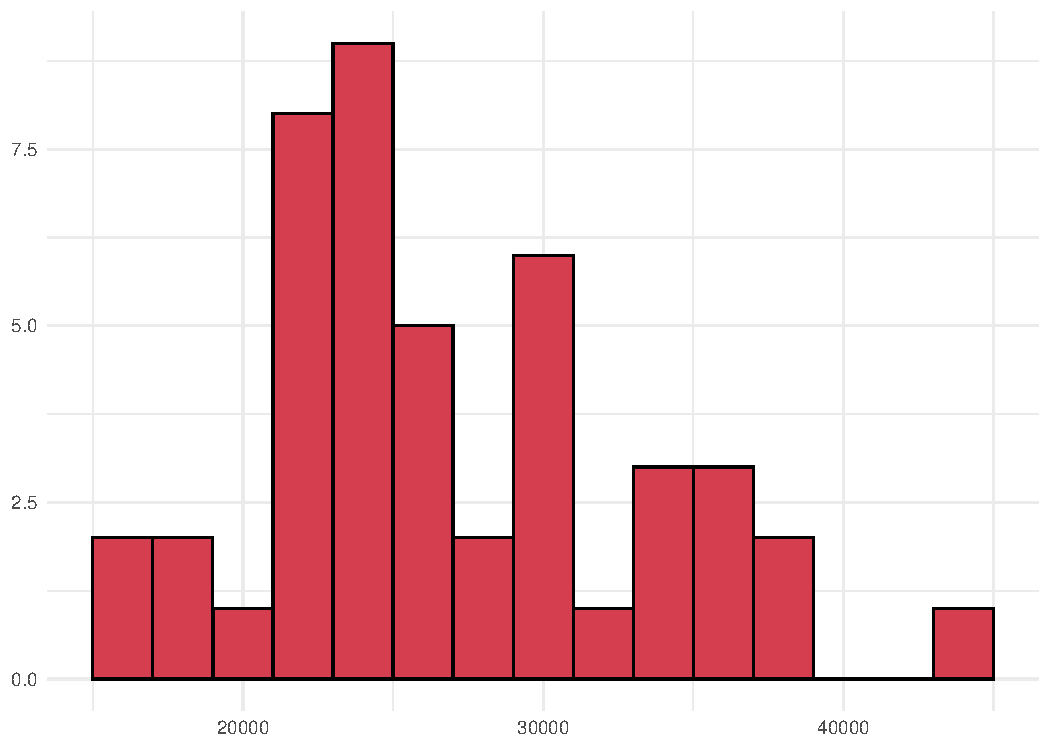
\includegraphics[width=0.75\textwidth]{./_StudyResults/orderingTimeHist}
	\caption{Histogramm der Zeit (ms) unterteilt in Gruppen zur Erledigung von Aufgabe 1: Zahlenfolge. Darstellungsgenauigkeit: 2000ms}
	\label{fig:orderingTimeHistogram}
\end{figure}

\todoTob{Median etc time für einzelne gruppen tabelle?}

Bei der zweiten Aufgabe gibt es eine größeren gemessenen Zeitbereich, was unter Anderem daran lag, dass die Probanden oft lang gebraucht haben die Aufgabenstellung zu lesen bzw. zu verstehen. Der schnellste Teilnehmer beendete die Aufgabe nach 13.87 Sekunden. Durchschnittlich haben die Probanden knapp 35 Sekunden zur Aufgabenbewältigung gebraucht. Das Maximum 83.31 Sekunden Bearbeitungszeit liegt in großem Abstand zum 'Zweitlangsamsten', welcher bei knapp unter 50 Sekunden liegt. Ein starker Häufungspunkt um die 20 Sekunden Marke kann man gut in Abbilung~\ref{fig:matchingTimeHistogram} erkennen. 
Beim Vergleich der Gruppen sieht man, dass die \textbf{XX} Gruppe im Schnitt am schnellsten mit der Bearbeitung der Aufgabe fertig war. Einzelne Teilnehmer der Fade 5 Gruppe haben länger als die Meisten gebraucht, wohingegen die Probanden aus der Fade 20 Gruppe alle zwischen 19 und 24 Sekunden gebraucht haben. Insgesamt hat die Alarm Gruppe im Vergleich zu den Licht Gruppen Teilnehmer gehabt, die alle unter 32 Sekunden zur Bewältigung der Aufgabe benötigt haben.

\begin{figure}[H]
	\centering
	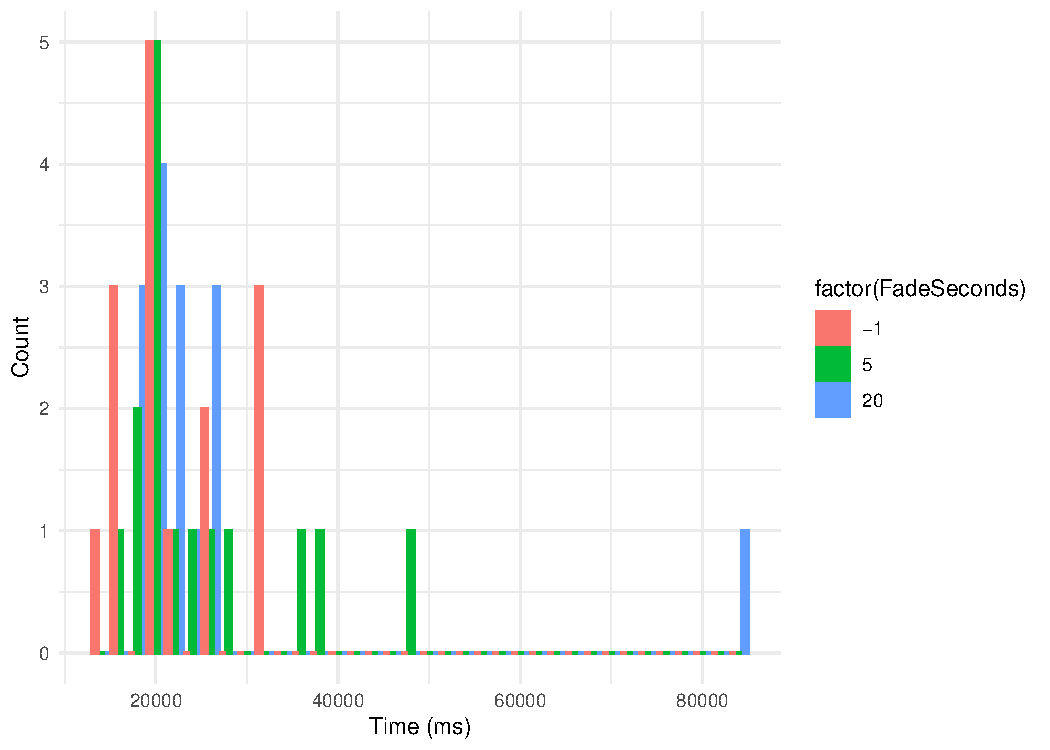
\includegraphics[width=0.75\textwidth]{./_StudyResults/matchingTimeHist}
	\caption{Histogramm der Zeit (ms) unterteilt in Gruppen zur Erledigung von Aufgabe 2: Stroop-Effekt. Darstellungsgenauigkeit: 2000ms}
	\label{fig:matchingTimeHistogram}
\end{figure}

Zum Bearbeiten der letzten Aufgabe wurden durchschnittlich 32.75 Sekunden gebraucht. Der schnellste Proband war in 15.34 Sekunden fertig und der langsamste Teilnehmer hat 54.15 Sekunden zur Absolvierung benötigt. Da die drei Teilaufgaben immer schwerer wurden, wurde im Vergleich immer mehr Zeit benötigt.
Wie in Abbildung~\ref{fig:countingTimeHistogram} einsehbar gibt es kaum Unterschiede der einzelnen Gruppen. Man kann erkennen, dass die Alarm Gruppe wieder etwas früher im Schnitt fertig war. \todoAll{hier mehr beschreiben nachdem vllt die tabelle da ist}

\begin{figure}[H]
	\centering
	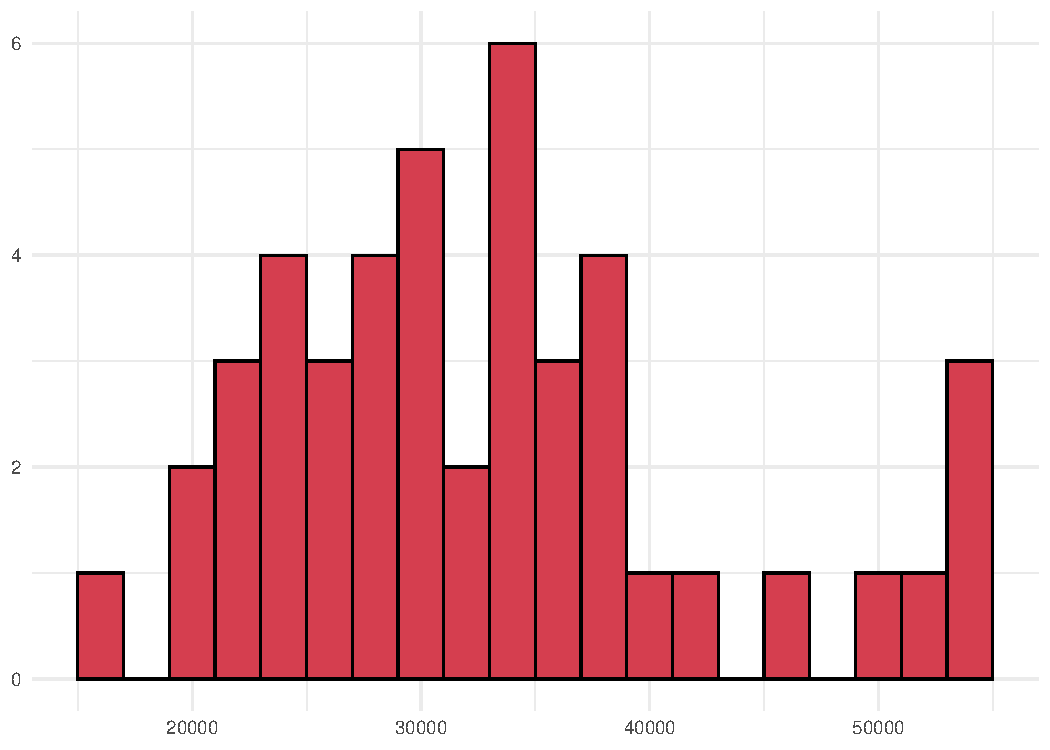
\includegraphics[width=0.75\textwidth]{./_StudyResults/countingTimeHist}
	\caption{Histogramm der Zeit (ms) unterteilt in Gruppen zur Erledigung von Aufgabe 3: Boxen zählen. Darstellungsgenauigkeit: 2000ms}
	\label{fig:countingTimeHistogram}
\end{figure}

Wenn man die Zwischenschritte aus Aufgabe 1 genauer betrachtet, kann man aus Abbildung~\ref{fig:timeTask1} entnehmen, dass nachdem die erste Zahlenblase zerplatzt wurde die zweite Blase innerhalb höchstens 3 Sekunden bei allen Gruppen betätigt wurde. Für die dritte und fünfte Blase ist ein Hochpunkt in allen drei Gruppen erkennbar, was zeigt, dass hier etwas mehr Zeit zur Sortierung benötigt wurde. Ab Zahlenblase sechs waren die Hälfte der Blasen weg, was für ein schnelleres Orientieren sorgt, was sich in den Zeiten wiederspiegelt. Gruppe Fade 5 benötigte im Schnitt etwa 1 Sekunde länger für das Auffinden, der fünften Blase. Darüberhinaus existieren keine großen Unterschiede der einzelnen Studiengruppen.
 
\begin{figure}[H]
	\centering
	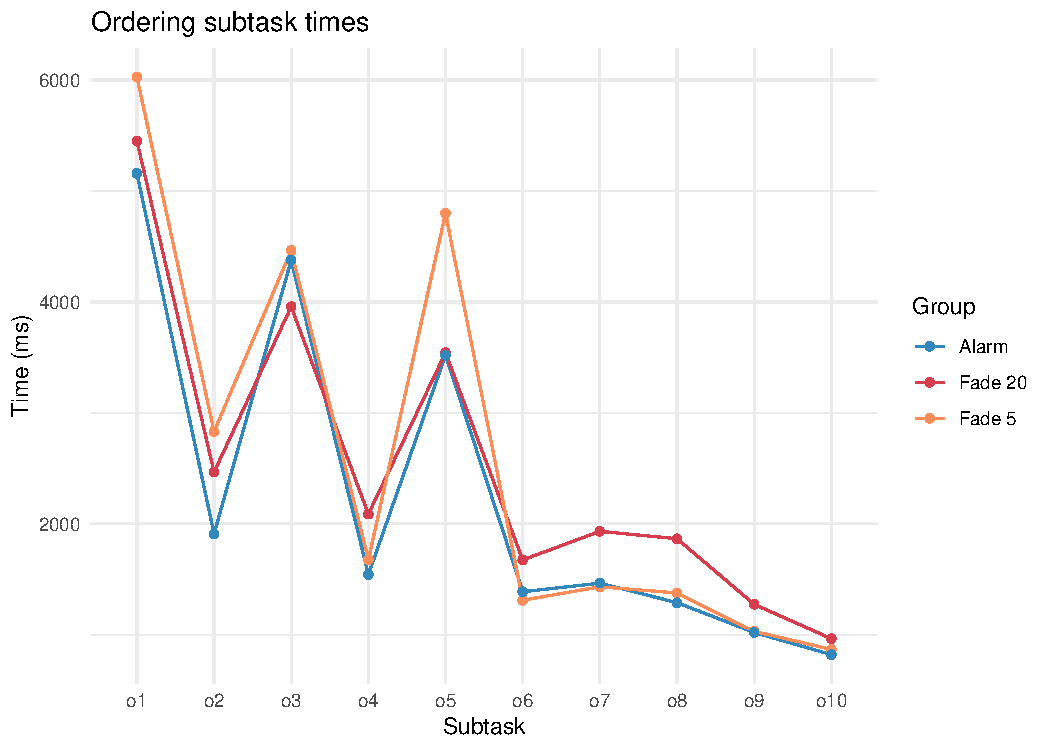
\includegraphics[width=0.75\textwidth]{./_StudyResults/timeTask1}
	\caption{Graph der einzelnen Zeiträume zwischen den Zwischenschritten für Aufgabe 1: Zahlenfolge}
	\label{fig:timeTask1}
\end{figure}

Bei Aufgabe 2 wurden die Zwischenschritte der einzelnen Teilaufgaben ebenso analysiert. In Abbildung~\ref{fig:timeTask2} erkennt man, dass die Fade 5 Gruppe im Schnitt nach 4 Sekunden, also am spätesten im Vergleich, mit Betätigen der ersten Farbblase angefangen hat. Ansonsten bewegen sich die Ergebnisse der drei Gruppen gleichmäßig mit einem Schwankungsbereich von 0.5 Sekunden.

\begin{figure}[H]
	\centering
	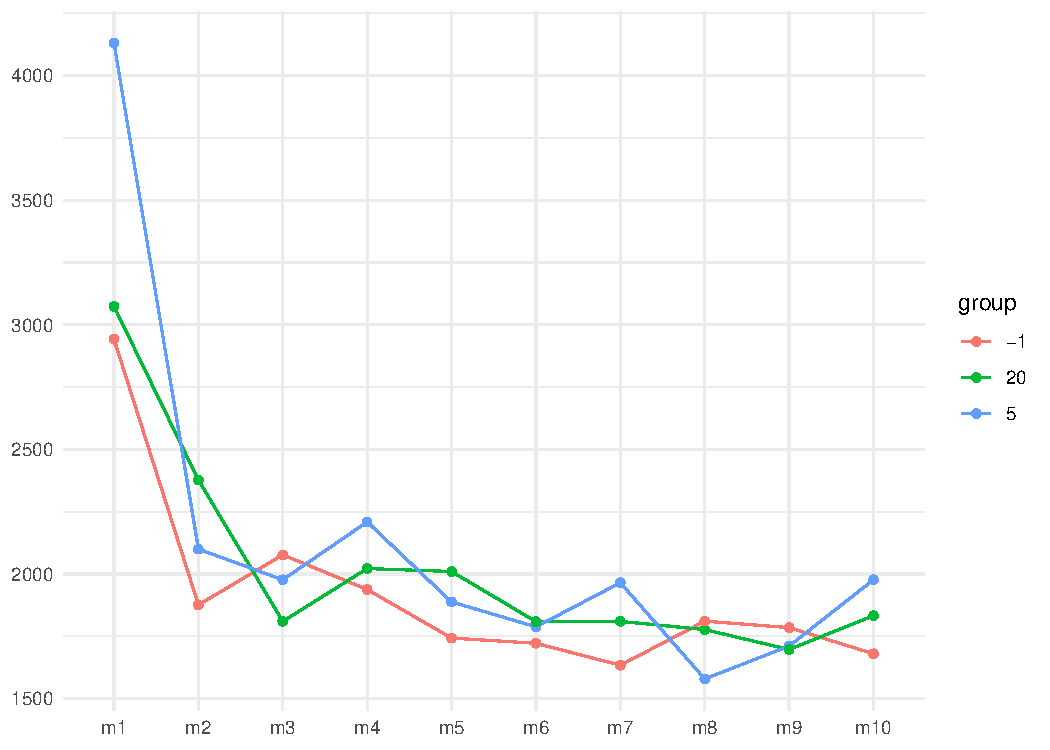
\includegraphics[width=0.75\textwidth]{./_StudyResults/timeTask2}
	\caption{Graph der einzelnen Zeiträume zwischen den Zwischenschritten für Aufgabe 2: Stroop-Effekt}
	\label{fig:timeTask2}
\end{figure}

In der Aufgabe des Boxenzählens wurden ebenso die Zwischenzeiten der Teilaufgaben gemessen wie in Abbildung~\ref{fig:timeTask3} zu sehen ist. Die Alarm Gruppe hat die erste Teilaufgabe am schnellsten beantwortet. Diese Gruppe hat im Schnitt ca 8 Sekunden für die erste Zahlenblase gebraucht und dann kontinuierlich, sogar fast linear länger pro Teilaufgabe gebraucht. Im Gegensatz dazu haben die anderen beiden Gruppen Fade 20 und Fade 5 fast 10 Sekunden für die erste Teilaufgabe gebraucht und verbesserten die Zeit bis zur letzten Betätigung der Zahlenblase. Die Gruppe Fade 20 hat am längsten für die zweite Aufgabe gebraucht aber war dafür am schnellsten bei der letzten Teilaufgabe.

\begin{figure}[H]
	\centering
	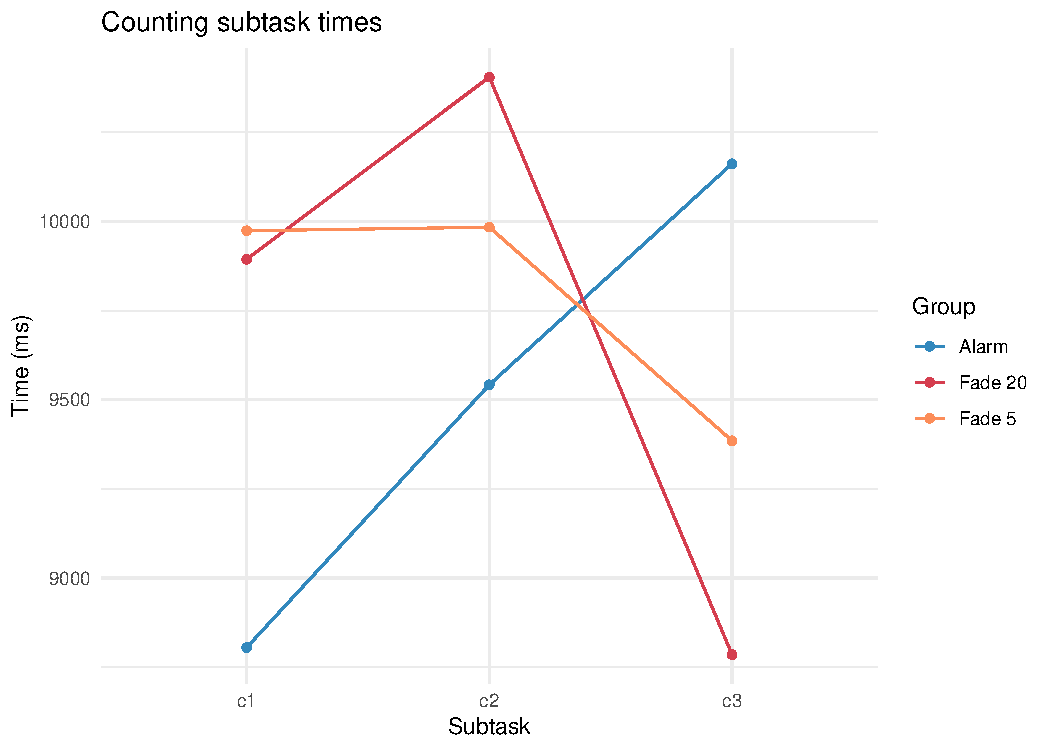
\includegraphics[width=0.75\textwidth]{./_StudyResults/timeTask3}
	\caption{Graph der einzelnen Zeiträume zwischen den Zwischenschritten für Aufgabe 3: Boxen zählen}
	\label{fig:timeTask3}
\end{figure}


\subsection{Selbsteinschätzungen, Fragebögen}\todoAll{subsection ggf umbennen}
%nur Vorschläge zur Gleiderung; hier sowas wie.. SAM, oder so..?

\todoTob{Ergebnisse: Kopfbewegungen}

\todoLuc{Abschnitt zu Ergebnisse von SAM schreiben}
Das Ausfüllen des SAM Fragebogen wurde einmal vor und einmal nach der Ruhephase verlangt. 

\begin{figure}[H]
	\centering
	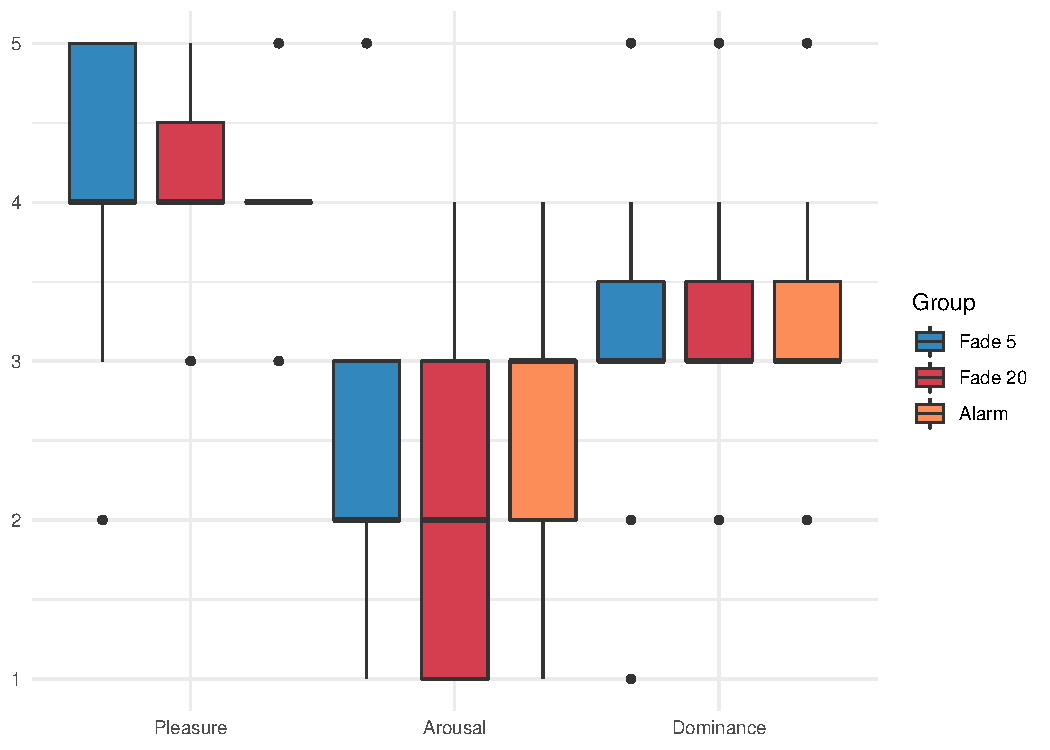
\includegraphics[width=0.75\textwidth]{./_StudyResults/SAMpre}
	\caption{Self-Assessment Manikin Ergebnisse vor der Ruhephase}
	\label{fig:samPre}
\end{figure}
\begin{figure}[H]
	\centering
	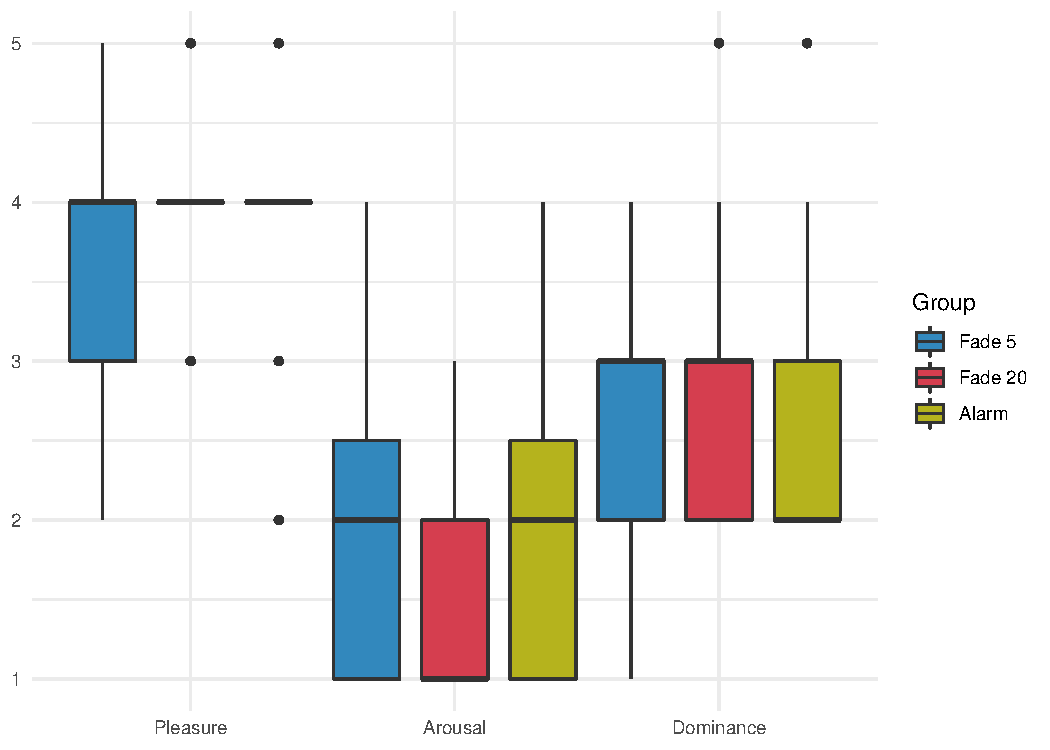
\includegraphics[width=0.75\textwidth]{./_StudyResults/SAMpost}
	\caption{Self-Assessment Manikin Ergebnisse nach der Ruhephase}
	\label{fig:samPost}
\end{figure}


Laut Befragung der Probanden im Anschluss an die Studie haben 20\% geschlafen, beziehungsweise mit den Teilnehmern, die fast geschlafen haben landet man bei 46,7\%. Ein geringer Prozentsatz hat meditiert und die anderen Nutzer gaben an nicht geschlafen zu haben, jedoch waren hier die meisten laut eigener Aussage trotzdem sehr entspannt. Genaue prozentuale Anteile können der Tabelle~\ref{tab:sleepstatus} und Abbildung~\ref{fig:slept} entnommen werden.

\begin{figure}
	\centering
	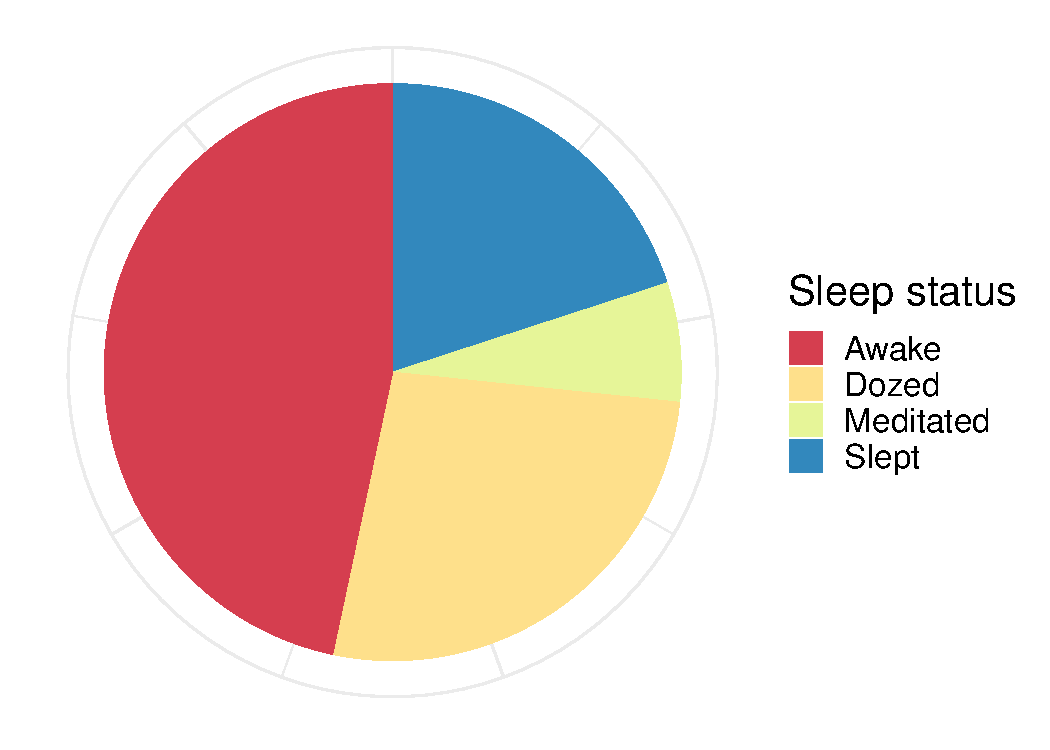
\includegraphics[width=0.75\textwidth]{./_StudyResults/slept}
	\caption{Subjektive Einschätzung der Dauer der Schlafphase}
	\label{fig:slept}
\end{figure}

Die empfundene Schlafdauer variiert in einem Zeitintervall zwischen 8 und 30 Minuten, wobei ein deutlicher Häufungspunkt bei der 15 Minuten Dauer anfällt und die 30 Minuten Angabe ein einzelner Ausreißer ist. Eine genaue Auflistung der Zeitangaben kann in Tabelle~\ref{tab:sleepduration} und Abbildung~\ref{fig:subjectiveSleepDuration} eingesehen werden.

\begin{figure}
	\centering
	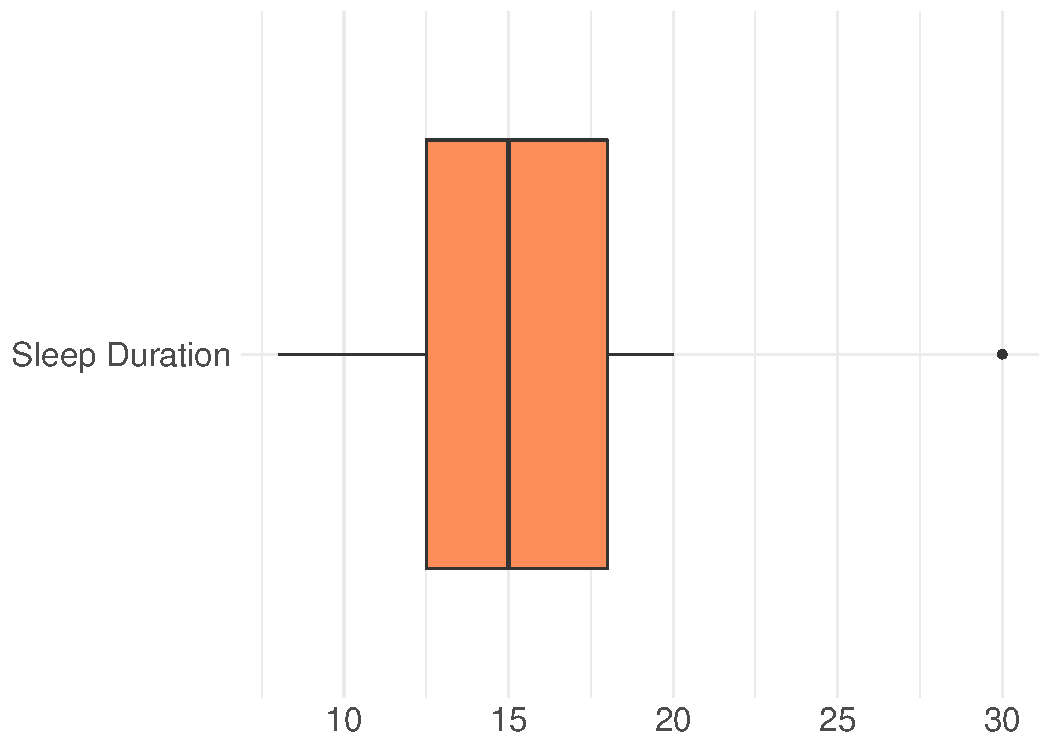
\includegraphics[width=0.75\textwidth]{./_StudyResults/subjectiveSleepDuration}
	\caption{Subjektive Einschätzung der Dauer der Schlafphase}
	\label{fig:subjectiveSleepDuration}
\end{figure}

\begin{figure}
	\centering
	\begin{subfigure}{0.48\textwidth}
		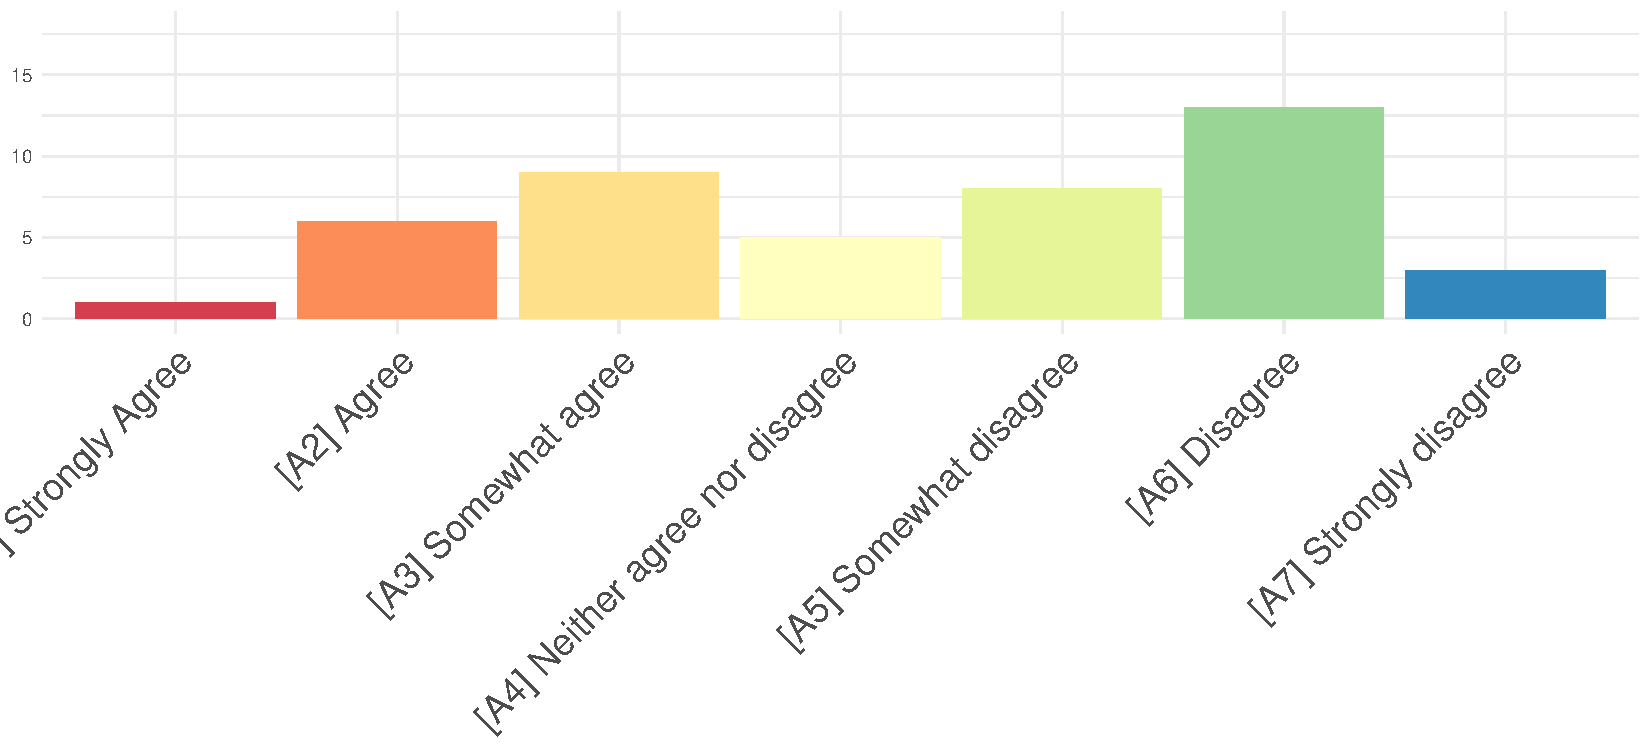
\includegraphics[width=\textwidth]{./_StudyResults/tiredBefore}
		\caption{Tired before}
		\label{fig:tiredBefore}
	\end{subfigure}%
	\hfill
	\begin{subfigure}{0.48\textwidth}
		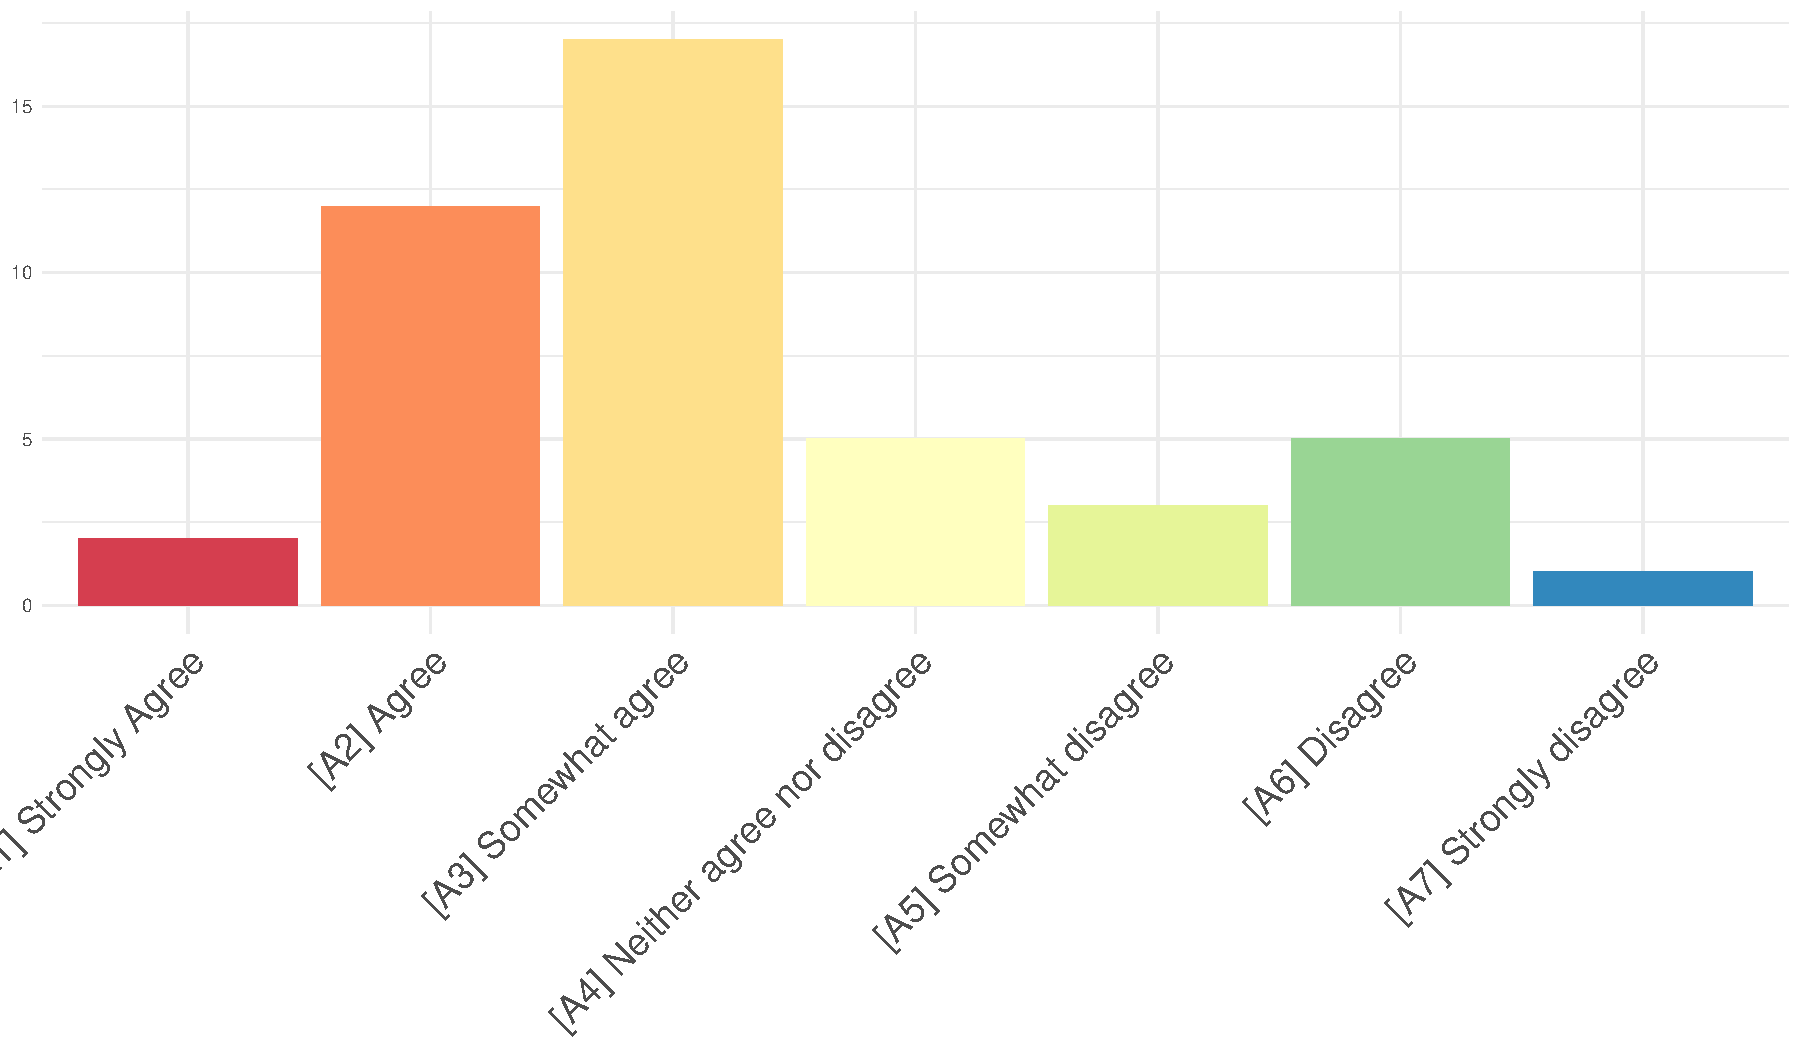
\includegraphics[width=\textwidth]{./_StudyResults/tiredAfter}
		\caption{Tired after}
		\label{fig:tiredAfter}
	\end{subfigure}
	\caption{Tired before and tired after} % caption for whole figure
\end{figure}

\begin{figure}
	\centering
	\begin{subfigure}{0.48\textwidth}
		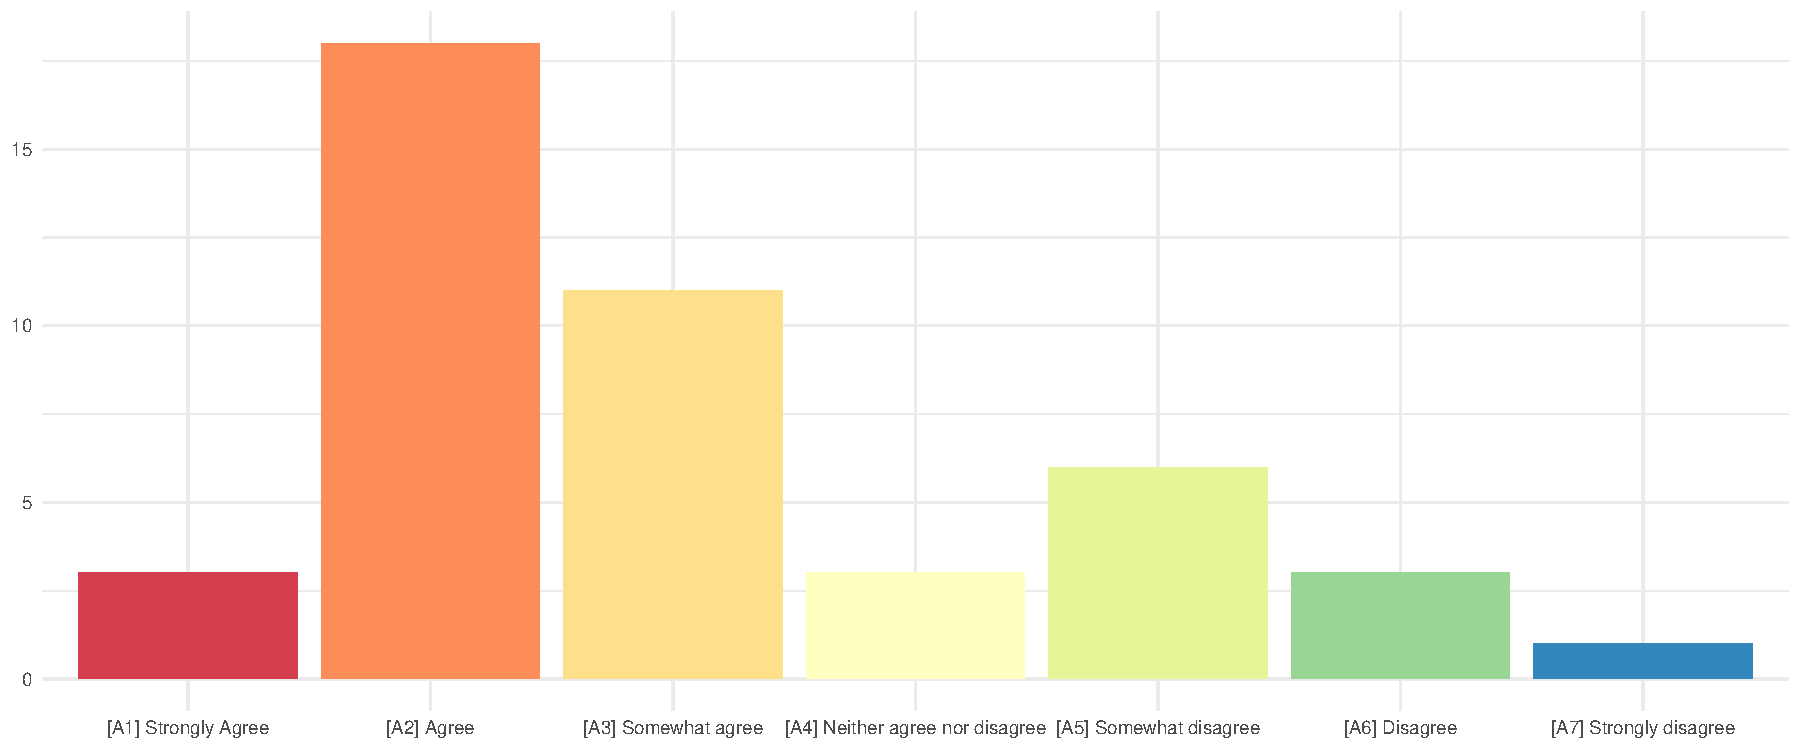
\includegraphics[width=\textwidth]{./_StudyResults/transitionEasy}
		\caption{Transition easy}
		\label{fig:transitionEasy}
	\end{subfigure}%
	\hfill
	\begin{subfigure}{0.48\textwidth}
		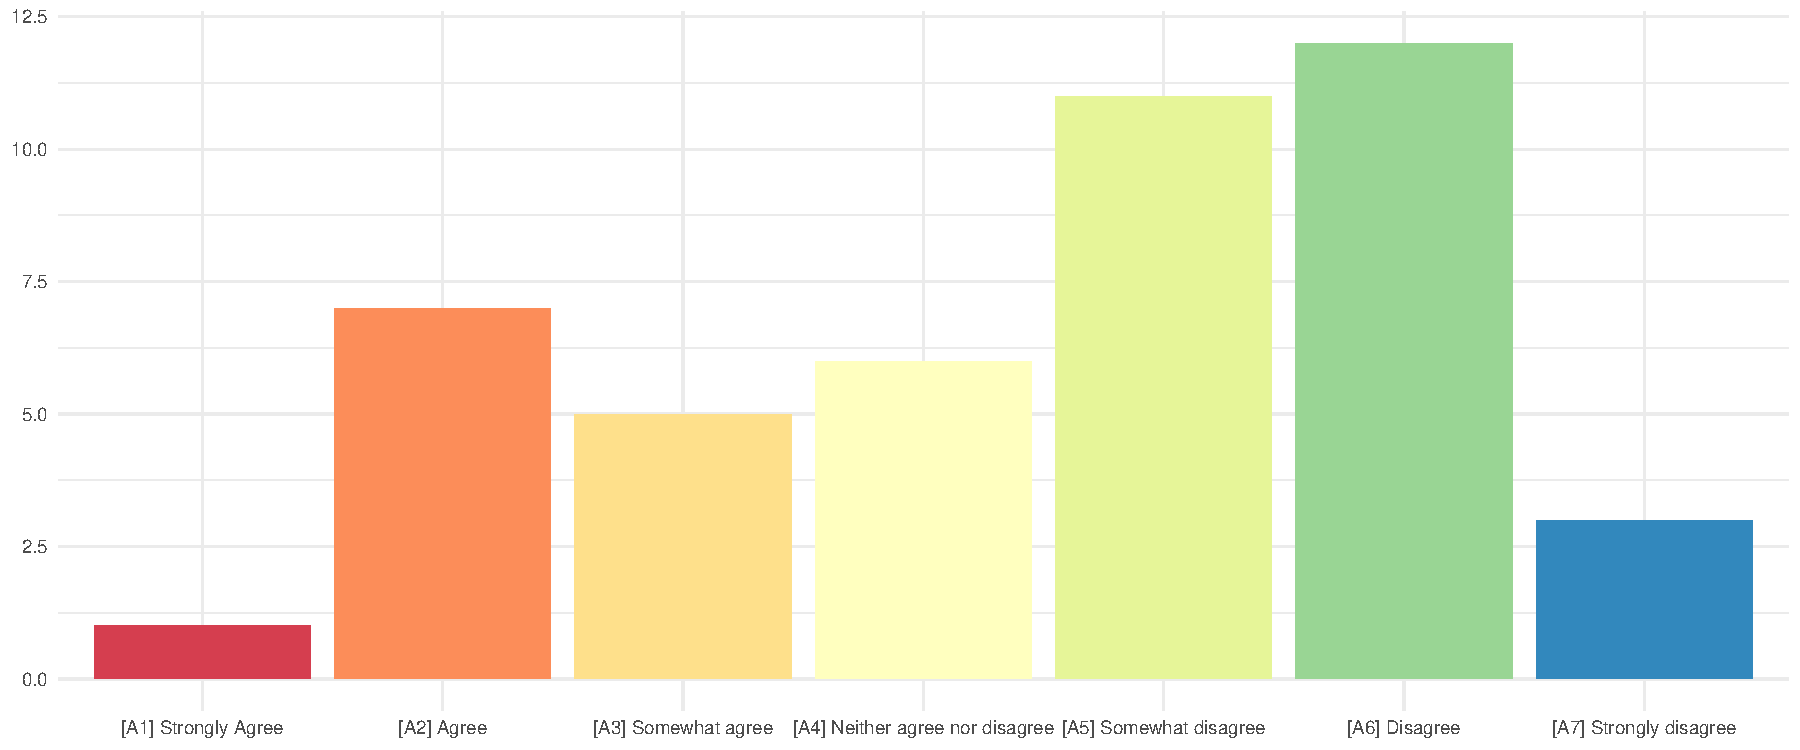
\includegraphics[width=\textwidth]{./_StudyResults/transitionHard}
		\caption{Transition hard}
		\label{fig:transitionHard}
	\end{subfigure}
	\caption{Transitions} % caption for whole figure
\end{figure}

\begin{figure}
	\centering
	\begin{subfigure}{0.48\textwidth}
		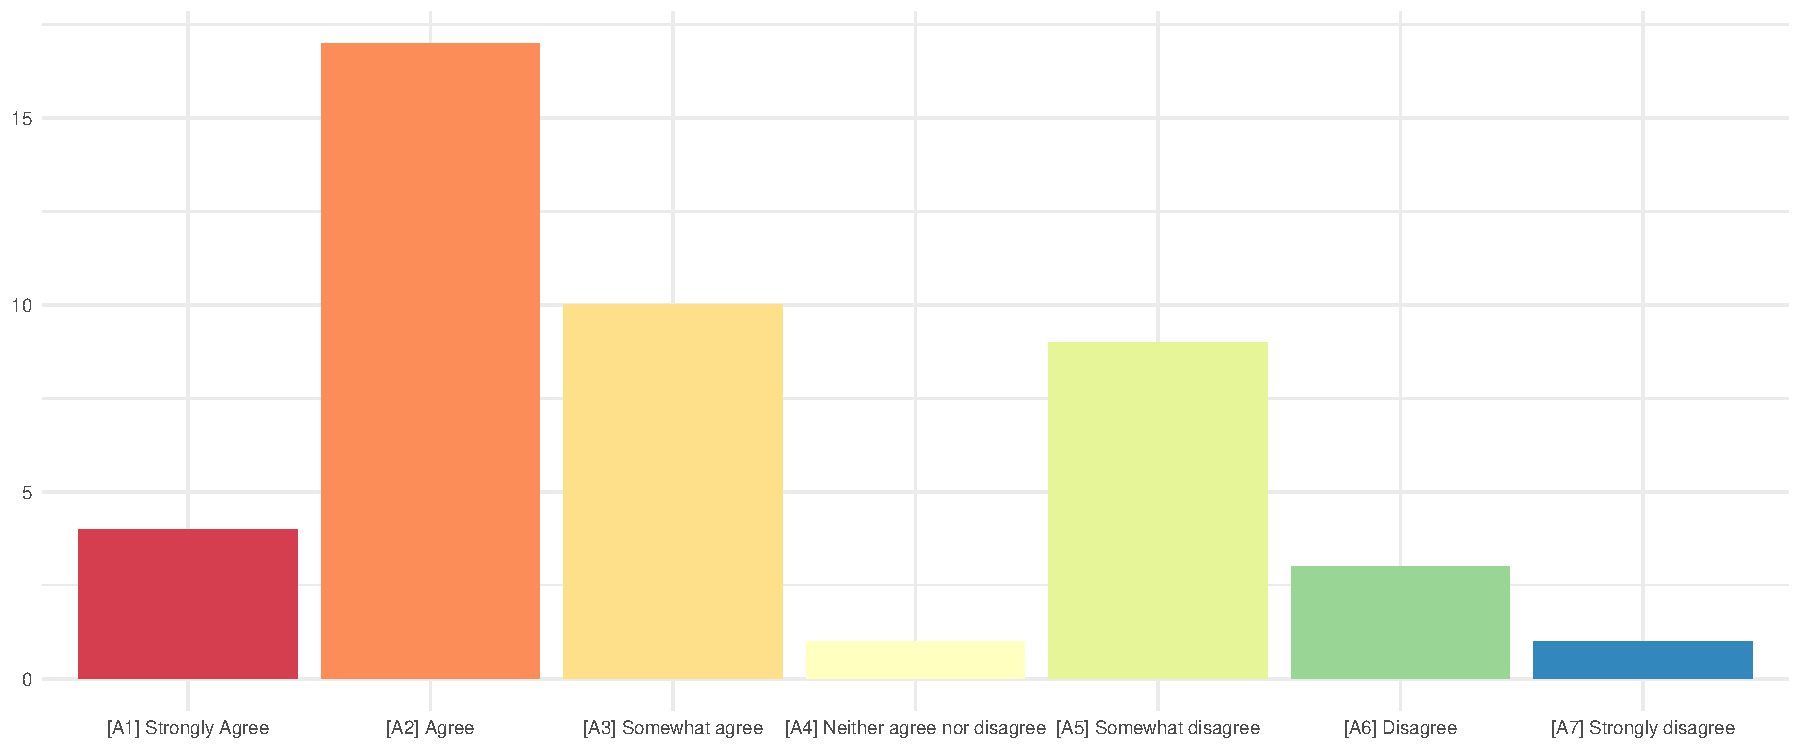
\includegraphics[width=\textwidth]{./_StudyResults/comfortableHeadset}
		\caption{comfortableHeadset}
		\label{fig:comfortableHeadset}
	\end{subfigure}%
	\hfill
	\begin{subfigure}{0.48\textwidth}
		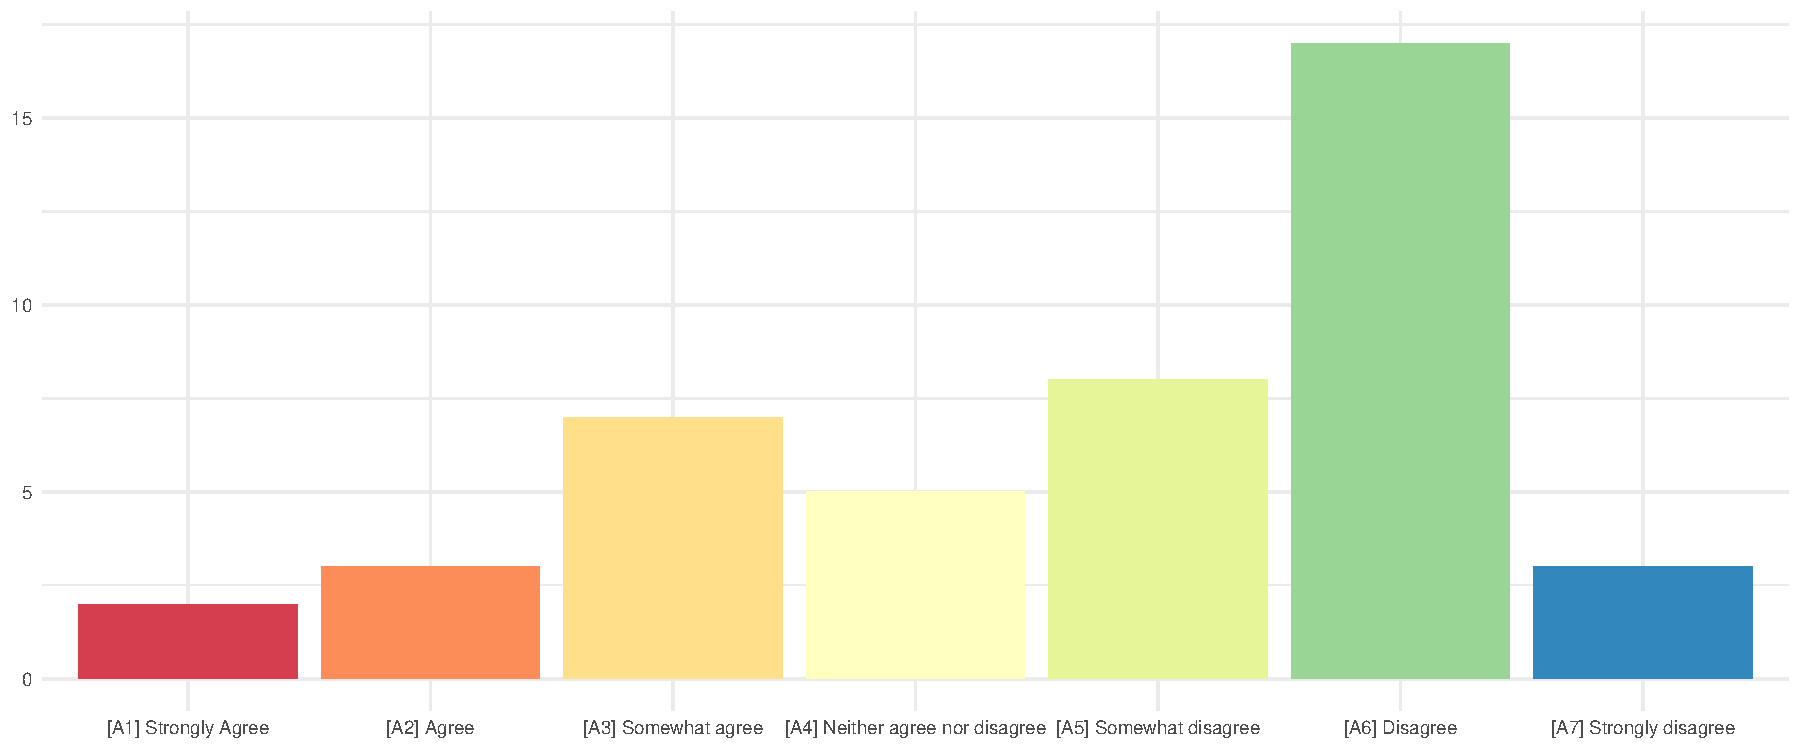
\includegraphics[width=\textwidth]{./_StudyResults/notComfortableHeadset}
		\caption{notComfortableHeadset}
		\label{fig:notComfortableHeadset}
	\end{subfigure}
	\caption{Headset comfort} % caption for whole figure
\end{figure}

\begin{figure}
	\centering
	\begin{subfigure}{0.48\textwidth}
		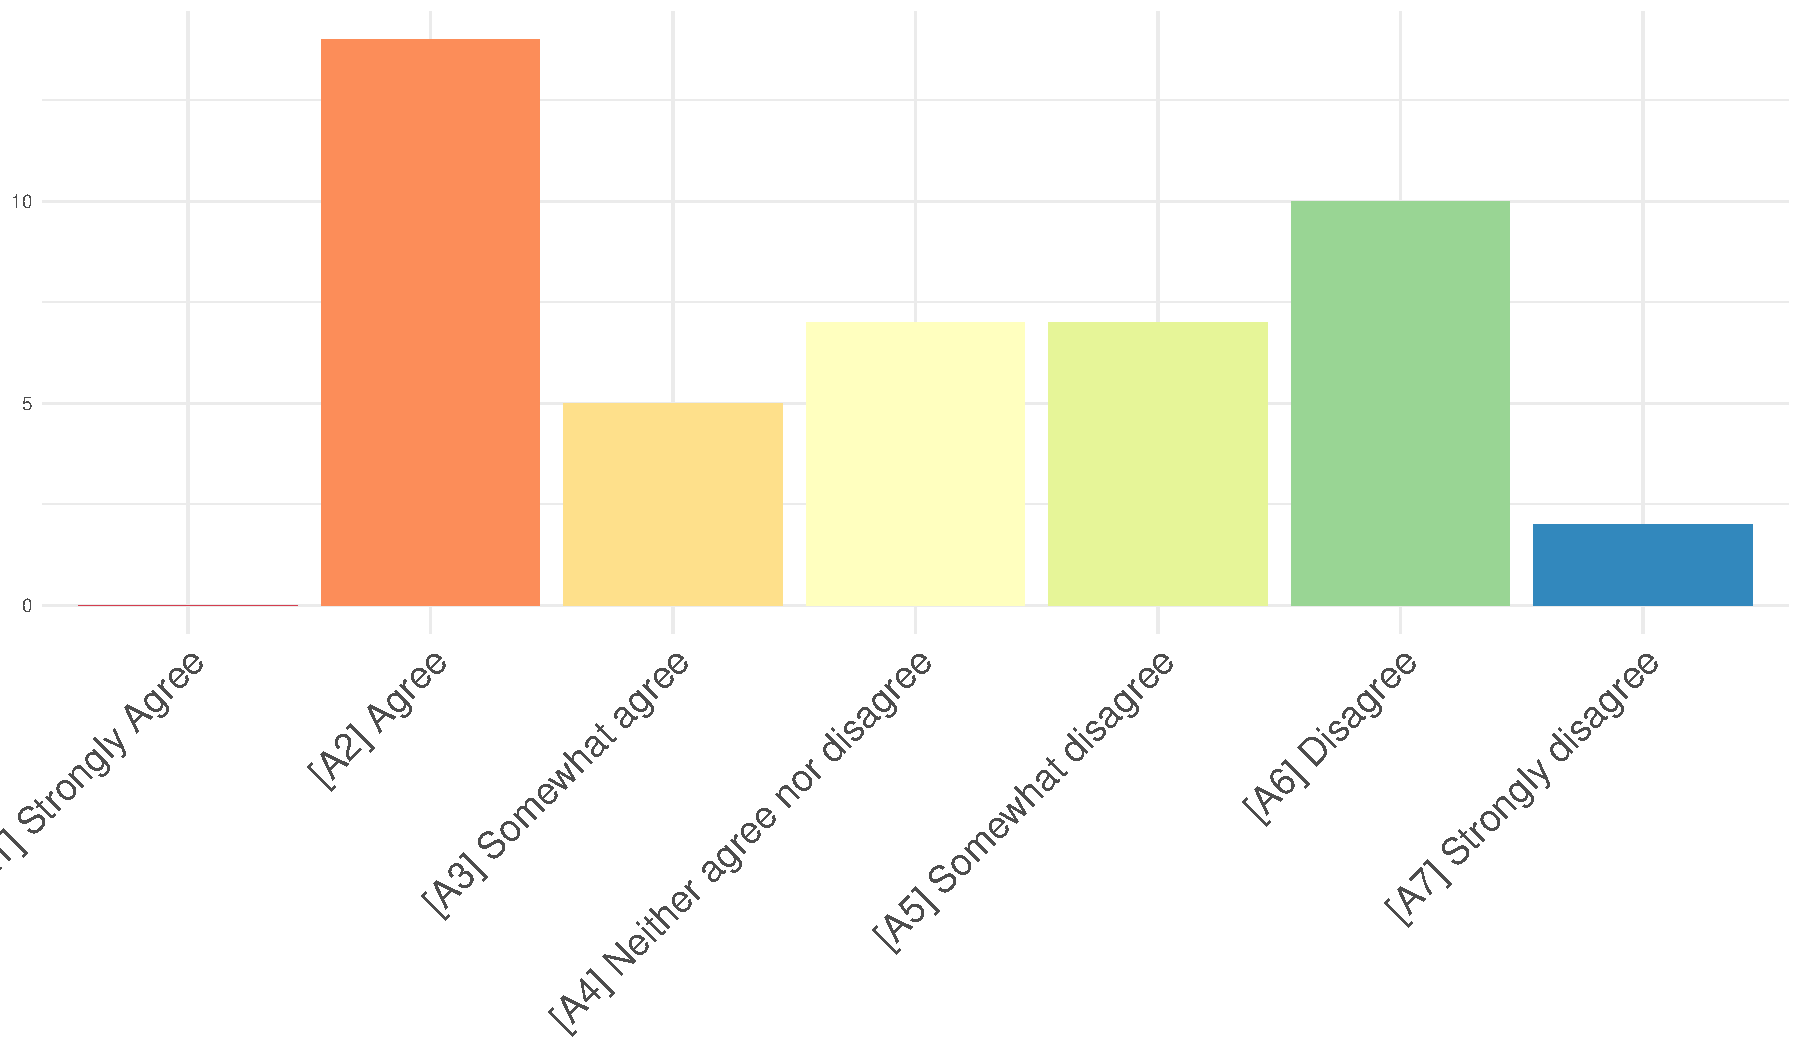
\includegraphics[width=\textwidth]{./_StudyResults/imagineWakingUp}
		\caption{imagineWakingUp}
		\label{fig:imagineWakingUp}
	\end{subfigure}%
	\hfill
	\begin{subfigure}{0.48\textwidth}
		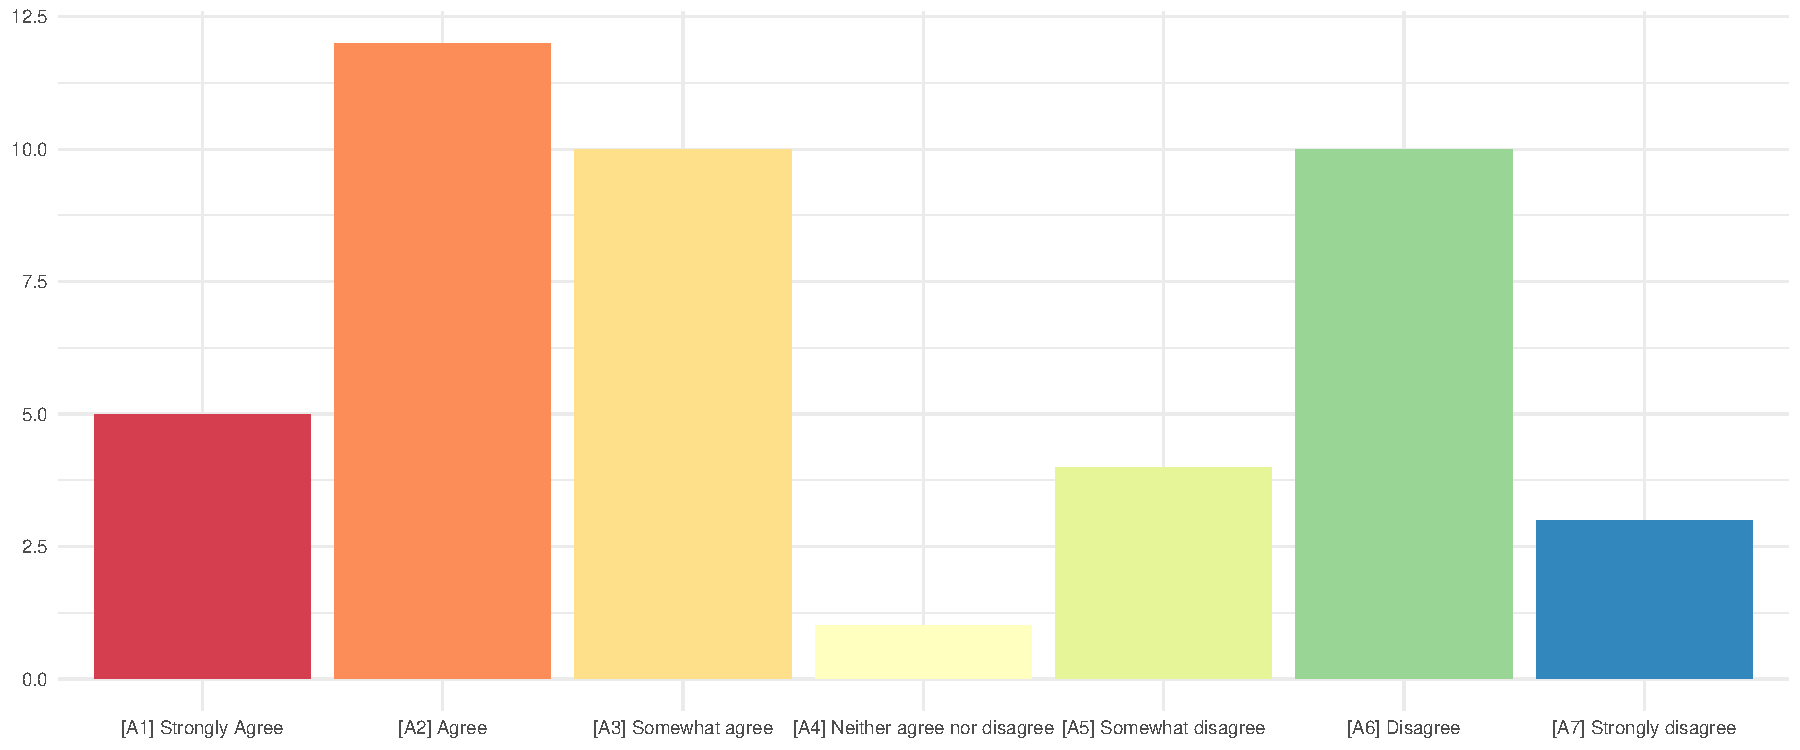
\includegraphics[width=\textwidth]{./_StudyResults/permanentWearing}
		\caption{permanentWearing}
		\label{fig:permanentWearing}
	\end{subfigure}
	\caption{Wearing} % caption for whole figure
\end{figure}

\begin{figure}
	\centering
	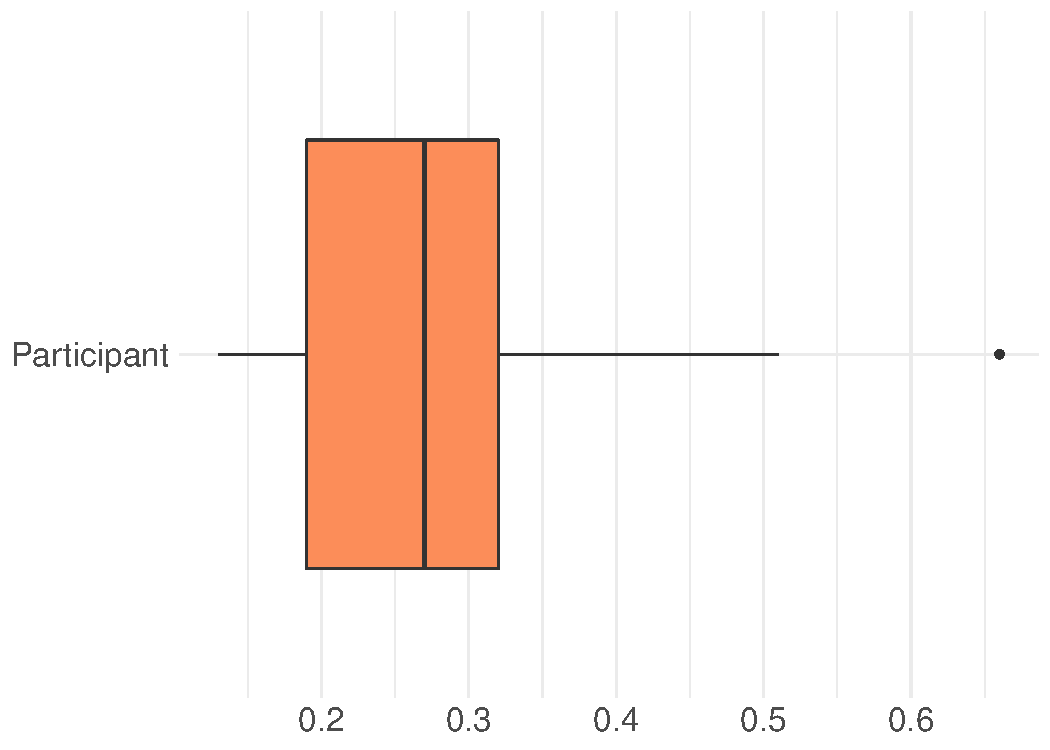
\includegraphics[width=0.75\textwidth]{./_StudyResults/rsme}
	\caption{RSME Visualisierung}
	\label{fig:rsme_vis}
\end{figure}


\chapter{Diskussion}
% -- hier ganz gute Beispiele zum Formulieren \url{https://www.scribbr.de/aufbau-und-gliederung/diskussion-beispiel/}
% --\\

Im Rahmen der Studie des Projekts \projectName \,haben die Ergebnisse unserer Untersuchung gezeigt, dass die Art und Weise des Aufwachens die anschließende Aufgabenbewältigung nicht signifikant beeinflusst.
Anhand der Ergebnisse und deren Interpretation gehen wir aber davon aus, dass weitere Untersuchungen durchaus signifikante Unterscheide hervorbringen könnten.

% Ist VR die richtige Herangehensweise?
Durch VR und AR können spezielle Situationen simuliert werden, die man einem Nutzer ohne diese Erweiterungen nicht darbieten könnte. Deshalb war es für uns die beste Möglichkeit ein konkretes Ruheszenario aufzubauen.

\chapter{Schlussfolgerung}

\todoAll{Schlussfolgerung Schreiben}
\todoAll{Wann wecken?}
\todoAll{Wie schnell wecken?}
\todoAll{Welche darstellung?}
\todoAll{Wie vorbereiten?}
\todoAll{Auf die Hypothesen eingehen}

Beachtet man die in Kapitel~\ref{cha:approach} aufgelisteten Hypothesen, so wird klar, dass keine der im voraus definierten Hypothesen komplett bestätigt wird. 
Zwar lässt sich beim Ordnen der Zahlen tatsächlich ein leichter Trend im Bezug auf Hypothese~\ref{hyp:lichtErfolgreicher} wahrnehmen, jedoch fällt diese nicht signifikant aus. 
Ansonsten lässt sich diese Hypothese jedoch nicht anhand er gesammelten Werte bestätigen. 
Hypothese~\ref{hyp:lichtSchneller} wird ebenfalls nicht durch die Werte bestätigt, da keine gravierenden Tendenzen zu beobachten sind.
Beim Stroop Test geht der Trend sogar eher in die Richtung, dass Menschen die mit einem akustischen Signal geweckt werden tendenziell eher etwas schneller sind und auch weniger Fehler machen als Probanden, welche einem Lichtreiz zum Wecken ausgesetzt wurden.
Dies spricht dementsprechend für die Gegenhypothese zu Hypothese~\ref{hyp:langKurzErfolgreicher}.

Auch in Bezug auf Hypothese~\ref{hyp:langKurzErfolgreicher} und~\ref{hyp:langKurzSchneller} lässt sich nicht herauslesen, dass eine der beiden Gruppen, welche mit Licht geweckt wurden bedeutsam besser oder schlechter als die andere Gruppe abgeschnitten hat. 
Den einzigen auszumachenden, wenn jedoch nicht besonders signifikanten, Unterschied erkennt man beim Ordnen der Zahlen. 
Hier zeigen die Daten, dass die Fade 5 Gruppe deutlichere Extrema im Bezug auf die Geschwindigkeit aufwiesen. 
Sowohl der schnellste als auch der langsamste gehörten dieser Gruppe an. 
Die Fade 20 Gruppe hingegen bewegt sich deutlicher im Mittelfeld der Grafik ~\ref{fig:orderingMistakeTimeScatterplot}.

\todoAll{Korrekturlesen}


\todos

\appendix		% Ab hier Appendices einbinden
\chapter{Anhang 1}

\begin{table*}
	\caption{Numerische Auflistung der Ergebnisse der Frage "`Please select your gender"'.}~\label{tab:sc_results_gender}
	
	\setlength\tabcolsep{3pt}
	\renewcommand{\arraystretch}{1.4}% for the vertical padding
	\begin{tabularx}{\textwidth}{ | x || r | r | }
		\hline
		Geschlecht & Absolutwerte 	& Prozentwerte \\ \hline\hline
		Männlich & 33 & 73.3\% \\ \hline
		Weiblich & 12 & 26.7\% \\ \hline
		Divers & 0 & 0.0\% \\ \hline
	\end{tabularx}
\end{table*}

\begin{table*}
	\caption{Numerische Auflistung der Ergebnisse der Frage "`Please enter your age in years"'.}~\label{tab:sc_results_age}
	
	\setlength\tabcolsep{3pt}
	\renewcommand{\arraystretch}{1.4}% for the vertical padding
	\begin{tabularx}{\textwidth}{ | x | x | x | x | x | x | }
		\hline
		Min & Max & Range & Median & Mean  & Standard Deviation \\ \hline\hline
		19  & 30  & 11    & 23     & 23.04 & 2.53              \\ \hline
	\end{tabularx}
\end{table*}

\begin{table*}
	\caption{Verteilung der Antworten zur Frage "`How much experience do you have with VR?"'.}~\label{tab:sc_results_expVR}
	
	\setlength\tabcolsep{3pt}
	\renewcommand{\arraystretch}{1.4}% for the vertical padding
	\begin{tabularx}{\textwidth}{ | x || r | r | }
		\hline
		Studienfach 						& Absolutwerte 	& Prozentwerte \\ \hline\hline
		[A1] No experience at all 			& 10 			& 22.2\% \\ \hline
		[A2] Almost no experience 			& 15 			& 33.3\% \\ \hline
		[A3] Less than average experience 	& 3 			& 6.7\% \\ \hline
		[A4] Some experience 				& 10 			& 22.2\% \\ \hline
		[A5] More than average experience 	& 2 			& 4.4\% \\ \hline
		[A6] Experienced 					& 2 			& 4.4\% \\ \hline
		[A7] Very highly experienced 		& 3 			& 6.7\% \\ \hline
	\end{tabularx}
\end{table*}

\begin{table*}
	\caption{Numerische Auflistung der Ergebnisse der Frage "`How much experience do you have with VR?"'.}~\label{tab:sc_numbers_expVR}
	
	\setlength\tabcolsep{3pt}
	\renewcommand{\arraystretch}{1.4}% for the vertical padding
	\begin{tabularx}{\textwidth}{ | x | x | x | x | x | x | }
		\hline
		Min & Max & Range & Median & Mean  & Standard Deviation \\ \hline\hline
		1  & 7  & 6    & 2     & 2.93 & 1.78              \\ \hline
	\end{tabularx}
\end{table*}

\begin{table*}
	\caption{Verteilung der Antworten zur Frage "`How much experience do you have with AR?"'.}~\label{tab:sc_results_expAR}
	
	\setlength\tabcolsep{3pt}
	\renewcommand{\arraystretch}{1.4}% for the vertical padding
	\begin{tabularx}{\textwidth}{ | x || r | r | }
		\hline
		Studienfach 						& Absolutwerte 	& Prozentwerte \\ \hline\hline
		[A1] No experience at all 			& 17 			& 37.7\% \\ \hline
		[A2] Almost no experience 			& 10 			& 22.2\% \\ \hline
		[A3] Less than average experience 	& 7 			& 15.5\% \\ \hline
		[A4] Some experience 				& 8 			& 17.7\% \\ \hline
		[A5] More than average experience 	& 2 			& 4.4\% \\ \hline
		[A6] Experienced 					& 1 			& 2.2\% \\ \hline
		[A7] Very highly experienced 		& 0 			& 0.0\% \\ \hline
	\end{tabularx}
\end{table*}

\begin{table*}
	\caption{Numerische Auflistung der Ergebnisse der Frage "`How much experience do you have with AR?"'.}~\label{tab:sc_numbers_expAR}
	
	\setlength\tabcolsep{3pt}
	\renewcommand{\arraystretch}{1.4}% for the vertical padding
	\begin{tabularx}{\textwidth}{ | x | x | x | x | x | x | }
		\hline
		Min & Max & Range & Median & Mean  & Standard Deviation \\ \hline\hline
		1  & 6  & 5    & 2     & 2.36 & 1.38              \\ \hline
	\end{tabularx}
\end{table*}

\begin{table*}
	\caption{Verteilung der Antworten zur Frage "`What subject, if any, did you study or are you currently studying?"'.}~\label{tab:sc_results_study}
	
	\setlength\tabcolsep{3pt}
	\renewcommand{\arraystretch}{1.4}% for the vertical padding
	\begin{tabularx}{\textwidth}{ | x || r | r | }
		\hline
		Studienfach & Absolutwerte & Prozentwerte \\ \hline\hline
		Biologie & 1 & 2.2\% \\ \hline
		Informatik & 8 & 17.8\% \\ \hline
		Informationssystemtechnik & 1 & 2.2\% \\ \hline
		Mathematik & 1 & 2.2\% \\ \hline
		Medieninformatik & 18 & 40.0\% \\ \hline
		Physik & 3 & 6.7\% \\ \hline
		Psychologie & 2 & 4.4\% \\ \hline
		Software Engineering & 8 & 17.8\% \\ \hline
		Wirtschaftsmathematik & 1 & 2.2\% \\ \hline
		Wirtschaftsphysik & 2 & 4.4\% \\ \hline
	\end{tabularx}
\end{table*}

\begin{table*}
	\caption{Verteilung der Einstellungen des Stuhls.}~\label{tab:sc_results_chair}
	
	\setlength\tabcolsep{3pt}
	\renewcommand{\arraystretch}{1.4}% for the vertical padding
	\begin{tabularx}{\textwidth}{ | x || r | r | }
		\hline
		Winkeleinstellungen	in Grad	& Absolutwerte 	& Prozentwerte \\ \hline\hline
		0 							& 7 			& 15.6\% \\ \hline
		30 							& 23			& 51.1\% \\ \hline
		60	 						& 10 			& 22.2\% \\ \hline
		90							& 5 			& 11.1\% \\ \hline
	\end{tabularx}
\end{table*}

\begin{itemize}
	\captionof{anno}{Anmerkungen und Hinweise von Studienteilnehmern}
	\item "`Die Musik war sehr störend, um in einen Ruhezustand zu kommen"'
	\item "`Die VR Umgebung war schön gestaltet, aber die rumschwebenden Partikel waren eher verwirrend, ich dachte ich kann mit diesen interagieren"'
	\item "`Der Stuhl war sehr entspannend und bequem"'
	\item "`Es fiel mir schwer einzuschlafen, da ich zum 1. mal VR gemacht habe und dann neugierig war"'
	\item "`Die Musik war sehr angenehm"'
	\item "`Das lange gedrückt halten zur Interaktion war störend"'
	\item "`haptisches Feedback durch Controller wäre git gewesen"'
	\item "`Die Brille war sehr unangenehm"'
	\item "`Der Ton fürs Wecken hat mich erschrocken"'
	\item "`Mit meiner Brille war es unangenehm die VR Brille zu tragen"'
	\item ...\todoLuc{hier noch mehr Kommentare der Teilnehmer aufnehmen, was hat die Probanden gestört etc}
\end{itemize}

\begin{table*}
	\caption{Wahrgenommene Schlafdauer.}~\label{tab:sleepduration}
	
	\setlength\tabcolsep{3pt}
	\renewcommand{\arraystretch}{1.4}% for the vertical padding
	\begin{tabularx}{\textwidth}{ | x || r | r | }
		\hline
		wahrgenommene Schlafdauer in min& Absolutwerte & Prozentwerte \\ \hline\hline
		8						   	    & 2			   & 4.4\% \\ \hline
		10   					        & 5			   & 11.1\% \\ \hline
		11						   	    & 1 		   & 2.2\% \\ \hline
		12						   	    & 3			   & 6.7\% \\ \hline
		13							    & 2			   & 4.4\% \\ \hline
		14							    & 1			   & 2.2\% \\ \hline
		10-15	      					 & 3		 & 6.7\% \\ \hline
		15							    & 13		 & 28.9\% \\ \hline
		15-20							 & 1		 & 2.2\% \\ \hline
		17								 & 2		 & 4.4\% \\ \hline
		18								 & 3		 & 6.7\% \\ \hline
		18,5							 & 1		 & 2.2\% \\ \hline
		19								 & 1		 & 2.2\% \\ \hline
		20								 & 6		 & 13.3\% \\ \hline
		30								 & 1		 & 2.2\% \\ \hline
	\end{tabularx}
\end{table*}

\begin{table*}
	\caption{Verteilung der Antworten zur Frage "`Hast du geschlafen?"' .}~\label{tab:sleepstatus}
	
	\setlength\tabcolsep{3pt}
	\renewcommand{\arraystretch}{1.4}% for the vertical padding
	\begin{tabularx}{\textwidth}{ | x || r | r | }
		\hline
		Schlafmodus					& Absolutwerte 	& Prozentwerte \\ \hline\hline
		geschlafen 					& 9 			& 20.0\% \\ \hline
		gedöst/kurz vor eingeschlafen	& 12			& 26.7\% \\ \hline
		meditiert					& 3			& 6.7\% \\ \hline
		nicht geschlafen			& 21 			& 46.7\% \\ \hline
	\end{tabularx}
\end{table*}
\todoTob{Hier noch ne Tabelle um die Atmung auszuwerten?}


\backmatter %%%%%%%%%%%%%%%%%%%%%%%%%%%%%%%%%%%%%%%%%%%%%%%%%%%%%%%%%%%%%%%%%%

\listoffigures	% Abbildungsverzeichnis
\listoftables	% Tabellenverzeichnis

%\bibliographystyle{natdin}
\bibliographystyle{IEEEtranS}	% alternativer Stil
\bibliography{MCI-Resync-Documentation}

\cleardoublepage
\clearscrheadfoot
% \declaration		% Erklärung, siehe diplom-mi-eng.cls

\end{document}
